\documentclass[10pt,a4paper,sans, oneside]{book}
\usepackage[top=2cm, bottom=2cm]{geometry} % Reduce document margins

\usepackage{titlesec}
\titleformat{\chapter}[hang]{\normalfont\huge\bfseries}{\thechapter:}{1em}{}

% Table of contents formatting
\setcounter{tocdepth}{1}

% Section formatting
\renewcommand\thechapter{\Alph{chapter}}
\renewcommand\thesection{\thechapter.\arabic{section}}
\renewcommand\thesubsection{\thesection.\arabic{subsection}}
\renewcommand\thesubsubsection{\thesubsection.\alph{subsubsection}}
\titlespacing\chapter{0em}{-2em}{0em}
\titlespacing\section{0em}{2em}{0em}
\titlespacing\subsection{0em}{2em}{0em}
\titlespacing\subsubsection{0em}{2em}{0em}

\usepackage[utf8]{inputenc}
\usepackage{fontawesome5}
\usepackage{orcidlink}
\usepackage{fontawesome5}
\usepackage{academicons}

% Foreground & background color management
\usepackage{xcolor}

% Insertable PDFs
\usepackage{pdfpages}

% Hyperlinks and urls
\usepackage{hyperref}
\hypersetup{
    colorlinks=true,
    linkcolor=blue,
    filecolor=magenta,
    urlcolor=cyan,
    pdftitle={G. Stark - Academic Qualifications Portfolio},
    pdfpagemode=FullScreen,
}

\usepackage{url}

% Scientific SI units
\usepackage{siunitx}
\usepackage{hepnames}

% Multi-column & multi-row tables
\usepackage{multicol}
\usepackage{multirow}

% Formatting lists
\usepackage{enumitem}

% Fancy headers package
\usepackage{fancyhdr}
\usepackage[font={small}]{caption}
\usepackage[hang,flushmargin]{footmisc}
%\linespread{1.1}
\linespread{1}
\pagestyle{fancy}
\fancyhead{}
\fancyhf{}
\fancyhead[C]{Dr. Giordon Stark: Academic qualifications portfolio for Faculty of Science, Lund University}
%\fancyfoot[L]{Research activity}
\fancyfoot[L]{Dr. G. Stark \faIcon{deaf} $\cdot$ Lunds Universitet $\cdot$ Senior Lecturer PA2024/647\\[-0.2em]{\fontsize{10}{0}\mdseries\upshape Pronouns: point/he/him}}
\rfoot{\thepage}

% https://tex.stackexchange.com/a/117334
% use fancyhdr on chapter pages
\usepackage{etoolbox}
\patchcmd{\chapter}{\thispagestyle{plain}}{\thispagestyle{fancy}}{}{}

% Create a custom command for formatting my project descriptions
% Project name, time period, collaboration, location
\newcommand{\ProjectSummary}[5]{\noindent\textbf{#1} \hfill #2 \\ \textit{#3} \hfill \textit{#4} \\ \textit{Collaborating institutions:} #5 }

\newcommand{\Activity}[4]{\noindent\textbf{#1} \hfill #2 \\ \textit{#3} \hfill \textit{#4} }

% Custom command for recommenders
% Name, Institute, Email, Phone number
%\newcommand{\Recommender}[4]{\noindent\textbf{#1}, \textit{#2}, \faEnvelope~\href{mailto:#3}{#3}, \faMobilePhone~#4 }
\newcommand{\Recommender}[3]{\noindent\textbf{#1}, \textit{#2}, \href{mailto:#3}{#3} }

% Custom command for publications
\newcommand{\Publication}[5]{\noindent\colorbox{#1}{\textcolor{#2}{\textbf{#3}}}~#4 \\ #5}

% For numbering publications
\newcommand{\PubCite}[3]{\colorbox{#1}{\textcolor{#2}{\textbf{#3}}}}

% Footnotes
\renewcommand{\thefootnote}{\alph{footnote}}

% Drafting assistance
%\usepackage[doublespacing]{setspace}
%\usepackage{lineno}
%\linenumbers

%%::: Custom commands
% "None yet" and "none" tags for section headers
\newcommand{\noneyet}{\normalsize{\textit{-- none yet}}}
\newcommand{\none}{\normalsize{\textit{-- none}}}

\newcommand{\phonesymbol}{\faIcon{phone}\ }
\newcommand{\emailsymbol}{\faIcon{envelope}\ }
\newcommand{\addresssymbol}{\faIcon{location-arrow}\ }
\newcommand{\mobilesymbol}{\faIcon{mobile}\ }
\newcommand{\homepagesymbol}{\faIcon{link}\ }

\usepackage[backend=biber,sorting=none]{biblatex}
\addbibresource{bib/main.bib}

\title{\Huge Academic qualifications portfolio for Faculty of Science, Lund University}
\author{\Large Dr. Giordon H. Stark\ \faIcon{deaf}\ {\small\color{gray}(pronouns: point/he/him)}\\[1em]\faIcon{university} Santa Cruz Institute for Particle Physics, UC Santa Cruz, United States}
\date{}

% DOCUMENT ITSELF
\begin{document}
\maketitle

\tableofcontents

\vspace{1cm}
\noindent Section H (List of selected publications) and Section I (All attachments and certificates) are uploaded separately, per the academic qualifications portfolio instructions.

\chapter{Cover Page \& Personal Letter}

\section{Cover Page} \label{sec:cover-page}
\noindent\makebox[\textwidth][c]{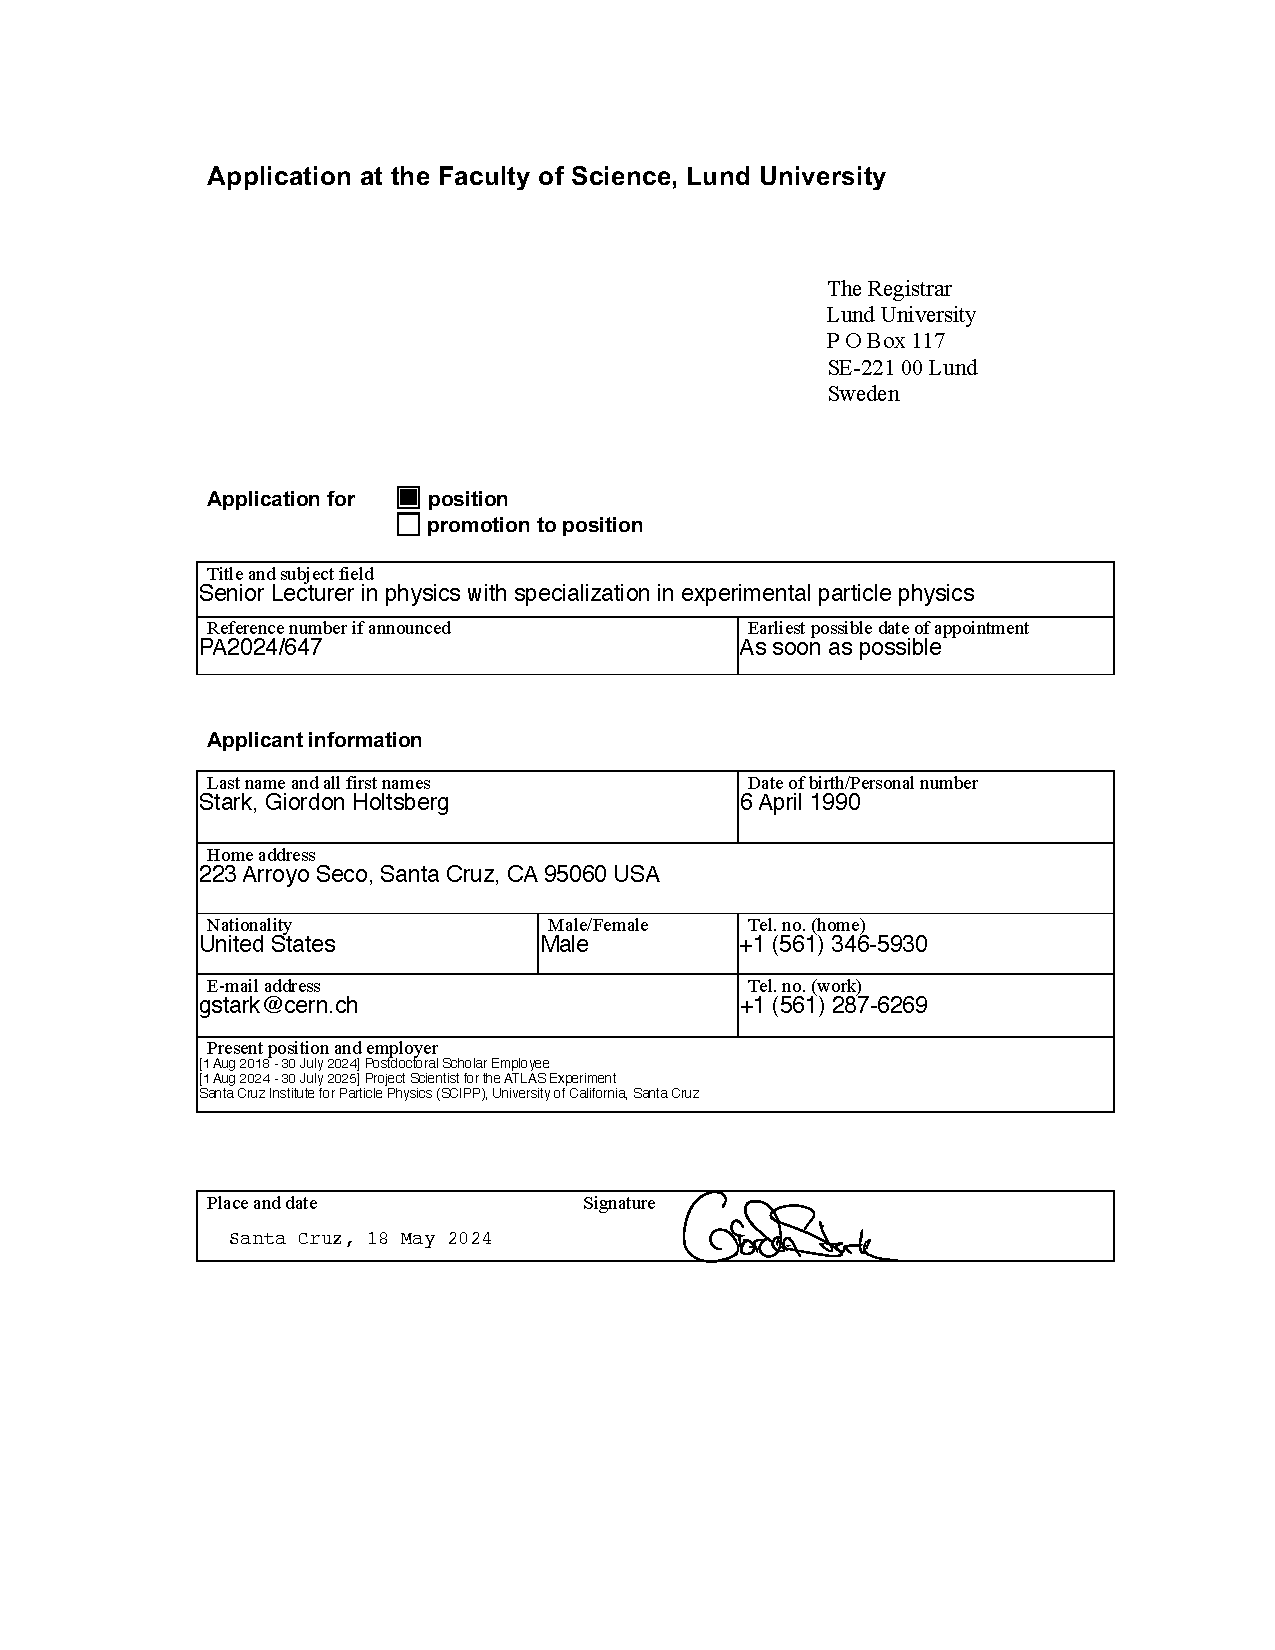
\includegraphics[width=1.1\textwidth]{attachments/cover-letter-academic-position-180928}}%

\clearpage
\section{Personal Letter} \label{sec:personal-letter}

\noindent Dear Prof. Lytken and the Lund Search Committee, \hfill \fcolorbox{black}{black!10}{May 25th, 2024}
\vspace{1em}

% TODO: maybe mention my leadership roles (ITk, Prod DB, FTF, DEI, etc)

I am attaching my application for the job position (\#PA2024/647) at Lunds universitet: \enquote{Universitetslektor i fysik med inriktning mot experimentell partikelfysik}. I found this position through a Swedish colleague. I obtained my Ph.D. in Physics from the University of Chicago in 2018 and am currently a postdoctoral scholar employee at the University of California, Santa Cruz, working on the ATLAS Experiment. Beginning August 1st, I transition to a Project Scientist position. I am thrilled at the prospect of continuing my work as a member of the ATLAS collaboration, my dedication to probing the fundamental questions of the Standard Model, and my passion for communicating my knowledge to Lund. My career in physics represents a commitment to the core value that Lund shares: widening participation for an inclusive University. In the attachments, I provide a diversity statement describing my unique background as a Deaf human in an oral world and how that shapes my passion for community outreach. And in both research and teaching, I work to provide a safe and inclusive environment so that my students, mentees, and colleagues can freely collaborate and foster new ideas. If appointed, my research program will be focused on Standard Model measurements, searches for new physics with the ATLAS experiment, instrumentation upgrades to support the completion of the HL-LHC physics program, and software development to meet the computing challenges of particle physics over the next decade.

At UChicago and UC Santa Cruz, I have been mentoring undergraduate students and graduate students across all of my research projects in hardware, software, and physics. Under my tutelage, I guided students through their physics analysis, supported them through struggles in their work-life balance, and worked with them to achieve their personal goals. For example, I was proud to mentor a graduate student, Dr. Jacob Pasner, who graduated from UCSC in 2019 with his Ph.D. on a search for boosted Higgs bosons. He finished his AAAS Fellowship in Washington, DC and now works for the State of California applying data science to water conservation efforts. I am also active in outreach activities, from giving international plenary talks to students in physics on how to advocate for their education and introducing LHC physics to local high schools through the QuarkNet and Masterclass programs. And finally, I was an active participant in the most recent Snowmass community effort to study the prospects of future colliders. My goal is to ensure a broad scope of work for myself and my students and continuity beyond the completion of the LHC program.

On a more personal note, one of the primary reasons for applying to this position is that I truly enjoyed the camaderie I experienced when I gave a seminar talk in September 2022 at your institution. I had a chance to talk with some of the current faculty there and appreciated the effort Lund invests in ensuring the success of all community members, both faculty and students alike. I feel that Lund will provide me the freedom to expand my current research activities and continue changing the status quo for modern particle physics, such as making ATLAS the first particle physics experiment to publish serialized, complete probability models for use by theorists, and as a teaching tool for statistics pedagogy.

Over the next decade, I plan to continue my close collaborations with various institutions and labs, including UChicago, UCSC, TUM, DESY, KTH, and IRIS-HEP, to support my research program. I am excited to keep working closely with the physics faculty and colleagues that I've worked with as a postdoc. As the first Deaf particle physicist, I am a very visual learner, and I have already been learning Swedish Sign Language for the past year. I am happy to provide any additional material upon request, in addition to the enclosed Academic Qualifications Portfolio.


\includegraphics[height=1cm]{attachments/signature}
\vfill%


\chapter{Curriculum Vitae}

\section{Contact Information} \label{sec:contact-information}
{
	\footnotesize
	Dr. Giordon Stark (point/he/him)~\orcidlink{0000-0001-6616-3433}                 \hfill \href{mailto:gstark@cern.ch}{\faIcon{envelope}~gstark@cern.ch}
	\vspace{0mm}\\\vspace{0mm}%
	UCSC SCIPP, 1156 High Street  \hfill \href{https://github.com/kratsg}{\faIcon{github}~kratsg} {\color{red!75!black!50}\large\rmfamily\textbullet} \href{{https://gitlab.cern.ch/gstark}}{\faIcon{gitlab}~gstark}
	\vspace{0mm}\\\vspace{0mm}%
	Natural Sciences 2, Room \#337       \hfill \href{{https://instagram.com/stark_baked}}{\faIcon{instagram}~kratsg} {\color{red!75!black!50}\large\rmfamily\textbullet} \href{skype:kratsg?chat}{\faIcon{skype}~kratsg}
	\vspace{0mm}\\\vspace{0mm}%
	Santa Cruz, CA \ \ \ 95064\hfill\href{https://giordonstark.com/?utm_source=cv}{\faIcon{external-link-alt}~https://giordonstark.com/}
}

\vspace{-2.0em}\section{Education} \label{sec:education}
{
	\footnotesize
	\textbf{University of Chicago}, Chicago, Illinois, US \hfill \textbf{Sep 2012 -- Jul 2018}\\
	\textsl{Supervisor}: David W. Miller \hfill \textsl{Degree}: M.S. Physics, Ph.D. Physics\\
	\href{https://kratsg.github.io/thesis/?utm_source=cv}{\faIcon{link}}~\textsl{The search for supersymmetry in hadronic final states using boosted object reconstruction} [\href{https://books.google.com/books?vid=ISBN978-3-030-34548-8}{\faIcon{book}~978-3-030-34548-8}]\\
	\textbf{Caltech}, Pasadena, California, US \hfill \textbf{ Sep 2008 -- Jun 2012}\\
	\textsl{Supervisor}: Kenneth Libbrecht and Harvey Newman \hfill \textsl{Degree}: B.S. Physics\\
	\href{https://www.dropbox.com/s/h0mpop96cn563bq/Thesis.pdf?dl=0}{\faIcon{link}}~\textsl{Optical Coating Brownian Thermal Noise in Gravitational Wave Detectors}
}

\vspace{-2.0em}\section{Employment} \label{sec:employment}\vspace{-1em}
\begin{table*}[h!]
	\footnotesize
	\begin{tabular}{r|lr}
		\centering
		\normalsize\textbf{2018-present} & \textbf{SCIPP, UC Santa Cruz} (US)                   &                  \\
		\hline
		2024-present                     & Project Scientist (Experimental - ATLAS)             & 100\% research   \\
		2018-2024                        & Postdoctoral Scholar Employee (Experimental - ATLAS) & 100\% research   \\
		\hline\hline
		\normalsize\textbf{2012-2018}    & \textbf{University of Chicago} (US)                  &                  \\
		\hline
		2017-2018                        & Doctoral candidate                                   & 100\% research   \\
		2016-2017                        & Doctoral candidate                                   & 50\% research    \\
		2014-2016                        & Bridge Program Tutor                                 & 100\% teaching   \\
		2013-2015                        & Graduate research assistant (HEP)                    & 50\% research    \\
		2012-2013                        & Graduate research assistant (Atomic)                 & 50\% research    \\
		2012-2017                        & Graduate teaching assistant                          & 50\% teaching    \\
		\hline\hline
		\normalsize\textbf{2015-2016}    & \textbf{Brookhaven National Laboratory} (US)         &                  \\
		\hline
		2015-2016                        & US Dept of Energy SCGSR fellow                       & 100\% research   \\
		\hline\hline
		\normalsize\textbf{2012-2012}    & \textbf{Adaptly, NYC, NY} (US)                                          \\
		\hline
		2012-2012                        & Software Engineer                                    & 25\% CS research \\
		\hline\hline
		\normalsize\textbf{2008-2012}    & \textbf{California Institute of Technology}(US)      &                  \\
		\hline
		2012-2012                        & Undergraduate student instructor (Web Programming)   & 50\% teaching    \\
		2011-2012                        & Undergraduate research assistant (LIGO)              & 50\% research    \\
		2011-2011                        & Undegraduate teaching assistant (IST4)               & 25\% teaching    \\
		2010-2011                        & Undergraduate computational specialist (lab)         & 50\% teaching    \\
		2010-2010                        & Undergraduate research fellow (Submillimeter Waves)  & 100\% research   \\
		2010-2010                        & Undergraduate student instructor (Web Programming)   & 50\% teaching    \\
		\hline\hline
		\normalsize\textbf{~2011-2011}   & \textbf{Massachusetts Institute of Technology}(US)   &                  \\
		2011-2011                        & Undergraduate research assistant                     & 100\% research   \\
		\hline
	\end{tabular}
\end{table*}

\vspace{-2.5em}\section{Leave of absence \none}\label{sec:leave-of-absense-none}

\vspace{-0.0em}\section{Postdoc stays}\label{sec:postdoc-stays}
\textbf{SCIPP, UC Santa Cruz, US} \hfill Aug 2018 -- Jul 2024 \\
\textsl{Supervisor:} Prof.~Mike Hance \hfill 100\% research

\vspace{-2.0em}\section{Qualification for readership or equivalent \noneyet}\label{sec:qualification-for-readership-or-equivalent}
\, \\

\vspace{-4.5em}\section{Important assignments}\label{sec:important-assignments}
{
	\footnotesize
	\begin{tabular}{r|>{\bfseries}ll}
		\centering
		2018-present & core developer         & pyhf, ITk Pixel Modules QC/QA, ITk Production DB \\
		2023-2024    & Editorial Board member & VBF diHiggs to four $b$-quarks                   \\
		2018-2023    & core developer         & xAODAnaHelpers                                   \\
		2021-2022    & committee member       & ATLAS Early Career Scientist Board               \\
		2020-2022    & subconvener            & Supersymmetry: Run-2 Summaries                   \\
		2018-2022    & committee member       & US-ATLAS Diversity and Inclusion                 \\
		2019-2021    & contact person         & Common Dark Matter AMG-RECAST                    \\
		2018-2020    & contact person         & SUSY Combinations, SUSY Monte Carlo Production   \\
	\end{tabular}
}

% 2007-2008 & Youth Member of the Board of Directors of the Red Cross, Greater Palm Beach Area Chapter
% 2007-2008 & North County Committee Chair for the Greater Palm Beach Area American Red Cross
% 2006-2007 & Health \& Safety Education Chair for Youth Council for American Red Cross

\vspace{-2.0em}\section{Awards and distinctions}\label{sec:awards-and-distinctions}
{
	\footnotesize
	\begin{tabular}{r|l}
		May 2022         & UC Santa Cruz Outstanding Postdoctoral Fellow Award                              \\ % attachment
		Aug 2019         & Springer Thesis Award                                                            \\ % attachment
		Apr 2018         & CERN Fellowship (turned down)                                                    \\ % attachment
		May 2017         & Nathan Sugarman Award for Excellence in Graduate Student Research                \\ % attachment
		Jun 2016         & US ATLAS Outstanding Graduate Student Award                                      \\ % attachment
		Nov 2015         & Young Researchers’ Symposium Award for Best Poster Presentation                  \\ % attachment
		Oct 2015         & U.S. Department of Energy, Office of Science Graduate Student Research Fellowship \\ % attachment
		2013, 2014, 2015 & UChicago Excellence in Graduate Teaching nominee                                 \\ % TODO: FIND ME
		Nov 2014         & US LHC Users Association Lightning Round winner                                  \\ % attachment
		Jun 2012         & Caltech Excellent TA Award                                                       \\ % attachment, maybe don't add
		Jun 2010         & Edward C. and Alice Stone Fellow                                                 \\ % attachment
		Apr 2008         & Best of Class (Palm Beach Post)                                                  \\ % attachment
		Apr 2006         & Howard Shavel Youth Award (Red Cross)                                            \\ % attachment
		Apr 2006         & United States Achievement Academy All American Scholar At-Large Award Winner     \\ % attachment
	\end{tabular}
}

\vspace{-2.0em}\section{International research and teaching experience} \label{sec:international-research-and-teaching-experience}
{
\footnotesize
\textbf{Select ATLAS physics analysis projects} -- SUSY Electroweak pMSSM: Beijing IHEP (CN); Munich LMU (DE); Oxford (GB); ANL (US); Barcelona (ES); Tokyo ICEPP (JP); CERN (CH); Stockholm (SE) {\color{red!75!black!50}\large\rmfamily\textbullet} $\tilde{g}\tilde{g}\to tttt \to bbbb$: Victoria (CA); Sheffield (GB); Stony Brook (US); Bucharest IFIN-HH (RO); Barcelona (ES) {\color{red!75!black!50}\large\rmfamily\textbullet} Charginos to three leptons: Nikhef (NL); Oslo (NO); Adelaide (AU); Bologna (IT); UPenn (US) \\
\textbf{ATLAS Inner Tracker Upgrade} -- Pixels module testing:  CERN (CH); Tokyo ICEPP, KEK (JP); LPNHE, IJCLab, Saclay CEA (FR); Seigen, Bonn, G\"{o}ttingen, Munich (DE); Bologna, Genova, Milano, Trento (IT); Liverpool, Glasgow, Oxford (GB); LBL, UCSC, Oklahoma, ANL (US); Bergen (NO) {\color{red!75!black!50}\large\rmfamily\textbullet} Production Database (Pixels and Strips): KEK (JP); IFAE Barcelona, IFIC/CSIC-UV (ES); Genova, Milano (IT); TU Dortmund, MPP, DESY, Wuppertal, Bonn (DE); STFC, Glasgow, Liverpool, Sheffield, Oxford, Manchester (GB); SFU, TRIUMF, Montreal, Victoria, UBC, Carleton (CA); Lund (SE); Copenhagen (DK); Geneve, CERN, Bern (CH); CNRS (FR); Czech Academy of Sciences, Unicorn College (CZ); UPenn, ANL, LBNL, UCSC, Oklahoma, SLAC (US); PUJ (CO); JSI (SI); Johannesburg (ZA); INFN Genova (IT); LPNHE, IJCLab, Saclay CEA, APC, CNRS/IN2P3 (FR); Bergen, Oslo (NO); UWA (GR)
}

\vspace{-2.0em}\section{Assignments as editor, referee} \label{sec:assignments-as-editor-referee}
{
	\footnotesize
	JHEP (2022, 2020) {\color{red!75!black!50}\large\rmfamily\textbullet} SciPost Phys (2024 x2)
}

\vspace{-2.0em}\section{Scholarly/academic societies} \label{sec:scholarly-academic-societies}
\begin{tabular}{r|ll}
	2014-present & American Physical Society (APS) & \textit{member} \\
	2014-present & U.S.~LHC Users' Association     & \textit{member} \\
\end{tabular}

\vspace{-2.0em}\section{People who have earned a Ph.D.~degree or completed a postdoc stay under your supervision\noneyet} \label{sec:people-who-have-earned-a-phd-degree-or-completed-a-postdoc-stay-under-your-supervision--noneyet}
\, \\

\vspace{-4.5em}\section{References} \label{sec:references}
{
\footnotesize
\Recommender{Prof.~Mike Hance}{UC Santa Cruz}{mhance@ucsc.edu}\\
\Recommender{Prof.~St\'{e}phane Willocq}{UMass Amherst}{willocq@physics.umass.edu}\\
\Recommender{Prof.~David Miller}{UChicago}{David.W.Miller@uchicago.edu}\\
\Recommender{Dr.~Maria Elena Monzani}{SLAC}{monzani@slac.stanford.edu}\\
\Recommender{Prof.~Kyle Cranmer}{UWisconsin Madison}{kyle.cranmer@wisc.edu}\\
\Recommender{Prof.~Christian Ohm}{KTH}{chohm@kth.se}
}

\vspace{-2.0em}\section{Other relevant information of significance for the application} \label{sec:other-relevant-information-of-significance-for-the-application}
I am the first (culturally, big \enquote{D}) Deaf particle physicist in the world, the third Deaf person to get a Ph.D. in Physics internationally, and the first Deaf person with a Ph.D. in Physics outside of Europe.


\chapter{List of Selected Publications} \label{annotatedpapers}

The publications below are presented in reverse chronological order (newest first).
The DOI code is provided where possible.
I am author on all papers signed \textsl{ATLAS Collaboration} since 2015, and these can be viewed at \href{https://inspirehep.net/authors/1319078}{InspireHEP}.
Particle physics convention lists authors alphabetically.

\newcounter{publication}
\newcommand{\PubBase}[4]{\stepcounter{publication}\SelectedPublication{#1}{white}{\thepublication}{#2}{#3}{#4}}
\newcommand{\PubSoftware}[3]{\PubBase{darkgray}{#1}{#2}{#3}}
\newcommand{\PubExperiment}[3]{\PubBase{red}{#1}{#2}{#3}}
\newcommand{\PubFacilities}[3]{\PubBase{blue}{#1}{#2}{#3}}
\newcommand{\PubAccessibility}[3]{\PubBase{green!50!black}{#1}{#2}{#3}}
\newcommand{\PubTheory}[3]{\PubBase{magenta}{#1}{#2}{#3}}

\begin{center}
	\PubCite{darkgray}{white}{Software \& Computing}~\PubCite{red}{white}{Experiment}~\PubCite{magenta}{white}{Theory}~\PubCite{blue}{white}{Future Facilities}~\PubCite{green!50!black}{white}{Accessibility}
\end{center}

\PubSoftware{in-progress}{Formation Task Force for the CPSC, 2024 - in-progress}{\textit{Forming the Coordinating Panel for Software and Computing}, G. Stark et al.}
\begin{quotation}
	The Executive Committee of the Division of Particles and Fields (DPF) of the American Physical Society charged us to define the role and governance of a Coordinating Panel for Software and Computing (CPSC) to be hosted by DPF.
	I was honored ot be chosen as one of two Early Career members on this task force, compromised of nineteen members.
	This is in-progress, with a draft disclosed for the purposes of this application only, for the reviewers to understand the scope.
	This document that I have been involved in from January 2024 until June 2024 will define a new committee managed by DPF to coordinate the future of Software and Computing for U.S. High Energy Physics efforts in entirety.
	While all members contributed to all parts of the document equally in its current form, I was initially tasked with editing the \enquote{Implementation Strategies} section, and reviewing the \enquote{Career Development} and \enquote{Broaden Representation in S\&C} sections.
	When this is complete, it will be reviewed by the DPF Executive Committee, and modifications of the bylaws will occur and the CPSC will be formed as a new committee alongside CPAD (Coordinating Panel for Advanced Detectors).
\end{quotation}

\PubFacilities{10.48550/arXiv.2404.02100}{Limited Author, 2024 - pre-print}{\textit{Analysis Facilities White Paper}, G. Stark et al., arXiv:\texttt{\href{https://arxiv.org/abs/2404.02100}{2404.02100~[physics.hep-ex]}}.}
\begin{quotation}
	While this paper has not been peer-reviewed, I consider it important to me as one of my goals is to improve the accessibility of physics for all.
	I contributed to all of the discussions to define what a suitable Analysis Facility should look like to support future generations of physicists in the HL-LHC era, starting in 2029.
	My focus in this paper was primarily on the user-facing experience, streamlining the collaborative experience of an analysis team on a single set of resources, and ensuring that analysis work was preservable and reproducible.
\end{quotation}

\PubExperiment{10.21468/SciPostPhysCodeb.27}{First author, 2024 - journal article and code}{\textit{Reduce, reuse, reinterpret: An end-to-end pipeline for recycling particle physics results}, G. Stark et al., arXiv:\texttt{\href{https://arxiv.org/abs/2306.11055}{2306.11055~[physics.hep-ex]}}.}
\begin{quotation}
	I first started my postdoc tenure at UCSC in 2018 thinking about how far software has come.
	I surmised that it should be possible to run a full analysis \enquote{end-to-end} from generation to statistical analysis all in \faIcon{python}~\texttt{Python}.
	However, the tooling did not completely exist and I spent a lot of time working on other pieces of this pipeline in order to make this paper a reality.
	Finally, after about 5 years, all the steps were in place, and my supervisor and I had a good physics case for performing a reinterpretation -- particularly inspired by the $g-2$ results that came out of Fermilab.
	In addition, there was another ATLAS analysis searching for supersymmetry that we had published a few years prior for which I spent time getting the full probability model publicly available.
	Guided by our lofty vision, I sat down and fleshed out the entire \texttt{Python} package, \texttt{MaPyDe}, that would provide the functionality to exercise this pipeline.
	This paper presents the existence of this software package, in addition to two separate novel reinterpretations of existing ATLAS searches to demonstrate the efficacy, all done outside of the ATLAS collaboration.
	For this to be done outside of the ATLAS collaboration requires the full probability model or the detector acceptances and efficiencies for the analysis to be made public.
	Now, \texttt{MaPyDe} is used to quickly do reinterpretation, as well as being an approachable pedagogical tool for undergraduate education in particle physics.
\end{quotation}

\PubExperiment{10.48550/arXiv.2402.08347}{ATLAS Collaboration, 2024 - submitted to PRL}{\textit{A statistical combination of ATLAS Run 2 searches for charginos and neutralinos at the LHC}, G. Stark et al., arXiv:\texttt{\href{https://arxiv.org/abs/2402.08347}{2402.08347~[physics.hep-ex]}}.}
\begin{quotation}
	I started this analysis right at the beginning of my postdoc at UCSC.
	I was the Combinations contact person along with two others, and our job was to coordinate the analysis selections for the fourteen analyses that would eventually go into this paper.
	I spent a lot of time determining the statistical overlaps between the analyses, defining the harmonized object definitions and selections that all teams had to use, and provided recommendations on the treatment of the systematic uncertainties for all the teams.
	Once I became the convenever for the Run-2 Summaries physics subgroup, I appointed \enquote{ATLAS Analysis Contacts} who would help me see this through to publication.
	The team continued to focus on validating the probability models provided by the analysis teams and trying out various schemes for (de)correlating systematics between the channels, ascertaining their impact on the final results reported in the paper.
	In parallel, I worked to finalize the missing tooling needed to perform the statistical combinations properly and did some outreach with theorists to get them ready to be able to use the results of this paper once it was public.
	This paper is the first of its kind, paving the way to perform a statistical combination in particle physics, using probability models that have each been individually published by the corresponding analysis, and also provides the combined probability models used.
\end{quotation}

\PubExperiment{10.1007/JHEP05(2024)106}{ATLAS Collaboration, 2024 - journal article}{\textit{ATLAS Run 2 searches for electroweak production of supersymmetric particles interpreted within the pMSSM}, G. Stark et al., arXiv:\texttt{\href{https://arxiv.org/abs/2402.01392}{2402.01392~[physics.hep-ex]}}.}
\begin{quotation}
	The pMSSM efforts within ATLAS is a large-scale computational effort that attempts to probe a 19-parameter phenomenological minimal supersymmetric standard model.
	This analysis allows us to reuse existing ATLAS analyses that were designed to search for unphysical, simplified models by reinterpreting them and assessing their sensitivity to more physical scenarios predicted by supersymmetry.
	I helped lead the team during my convenership, designing the approach taken in the paper, as well as helping develop the software tooling that underlied the phase-space sampling needed to perform the reinterpretation.
	In addition, I migrated the internal ATLAS code for Monte Carlo production that the paper relied on to produce datasets for the team to use for analysis work.
	I also worked on the $g-2$ interpretations to summarize ATLAS' current sensitivity to probing the Standard Model measurement reported by Fermilab and ATLAS published this as two separate summary plots to use as reference.
	Finally, I worked on the particle-level analysis software that our team relied on to get these results out.
\end{quotation}

\PubExperiment{10.1140/epjc/s10052-023-11543-6}{ATLAS Collaboration, 2023 - journal article}{\textit{Search for supersymmetry in final states with missing transverse momentum and three or more b-jets in $139\ \mathrm{fb}^{-1}$ of proton–proton collisions at $\sqrt{s} = 13\ \mathrm{TeV}$ with the ATLAS detector}, G. Stark et al., arXiv:\texttt{\href{https://arxiv.org/abs/2211.08028}{2211.08028~[physics.hep-ex]}}.}
\begin{quotation}
	This is my thesis analysis and I was the lead analyzer.
	The analysis sets the strongest limits on the mass of gluinos (supersymmetric partners of the gluon) that we have today in particle physics.
	I was responsible for defining the signal, control, and validation regions for the discovery portion of the analysis, optimizing all of the kinematic selections for maximal sensitivity.
	I also wrote the entire statistical fitting procedure, came up with a novel approach for estimating the theoretical uncertainties that arise from the Monte Carlo generators, and uncertainties due to the estimation of the Standard Model backgrounds because of the data-driven normalization procedure I chose.
	Finally, I pioneered the first fully-preserved analysis code via RECAST (back in 2018) making this analysis the first in ATLAS to support the preservation efforts that are on-going today.
\end{quotation}

\PubAccessibility{10.48550/arXiv.2203.08748}{Limited Author, 2022 - Snowmass Whitepaper}{\textit{Accessibility in High Energy Physics: Lessons from the Snowmass Process}, G. Stark et al., arXiv:\texttt{\href{https://arxiv.org/abs/2203.08748}{2203.08748~[physics.ed-ph]}}.}
\begin{quotation}
	As the first Deaf physicist outside of Europe, I have and continue to face many barriers and wanted to provide some framework allowing others to make future events more accessible for people like myself.
	This paper was the work of the twelve of us who were invested in ensuring that the future of particle physics continued to remain inclusive, equitable, and accessible.
	My ability to contribute to the Snowmass Community Summer Study was inhibited by the lack of accessbility provided by the APS Division of Particles and Fields.
	I contributed to this paper, both through my personal experience suffering through this process, and also putting together concrete sets of recommendations to make events more inclusive.
	I helped frame the paper in the context of the Americans with Disabilities Act (ADA) of 1990 to highlight the shortcomings of the 30+ year-old law.
	Finally, I provided all information to accomodate persons from an auditory perspective -- describing all the different solutions that exist and pointing out the pros/cons for each solution to enable event organizers/management to make a decision that is equitable and appropriate for their participants.
	This paper was included as part of the final Snowmass proceedings and was used by the Particle Physics Project Prioritization Panel (P5) in their report to the U.S. funding agencies.
\end{quotation}

\PubTheory{10.21468/SciPostPhys.12.1.037}{Limited Author, 2021 - journal article}{\textit{Publishing statistical models: Getting the most out of particle physics experiments}, G. Stark et al., arXiv:\texttt{\href{https://arxiv.org/abs/2109.04981}{2109.04981~[physics.hep-ph]}}.}
\begin{quotation}
	Following the momentum of getting ATLAS to be the first particle physics experiment to release a full probability model, I continued to work closely with theorists and phenomenologists to define \enquote{best practices} and ensure maximal reuse of these results from experimental analyses.
	I contributed to the high-level discussions of that paper, from the perspective of an experimentalist trying to publish data, and coordinated this effort within the ATLAS Collaboration as I was a convener at the time.
	One thing I would like to point out with this publication is the call-out for \enquote{Infrastructure for open-world models} which is an area lacking effort and development, and part of my research program will be to improve this.
	In the paper below about \texttt{pyhf}, it should be clear that the infrastructure for \enquote{closed-world models} is relatively crowded, better understood, and less interesting for continued efforts.
\end{quotation}

\PubSoftware{10.1051/epjconf/202024506017}{Limited Author, 2020 - journal article}{\textit{Likelihood preservation and statistical reproduction of searches for new physics}, G. Stark et al.}
\begin{quotation}
	This is what I consider one of the most pivotal papers (and pieces of work), with two other colleagues of mine, working towards my goal of making physics more accessible.
	The three of us were core developers on a tool called \href{https://scikit-hep.org/pyhf/}{\texttt{pyhf}} which both provided a schema for the plain-text, machine-readable serialization of a class of mathematical likelihood functions called \texttt{HistFactory} in addition to a pure-\texttt{Python} implementation for performing statistical inference on these likelihood functions.
	The paper is a peer-reviewed version of a public note from ATLAS (\href{https://atlas.web.cern.ch/Atlas/GROUPS/PHYSICS/PUBNOTES/ATL-PHYS-PUB-2019-029}{\texttt{ATL-PHYS-PUB-2019-029}}) which announced the first full probability model published by the ATLAS Experiment.
	This paper marked the beginning of a paradigm shift, with well over 100+ citations of \texttt{pyhf} itself and welcomed with open arms by the theory/phenomenology communities, indicating the utility of making physics even more accessible.
\end{quotation}

%\PubExperiment{internal-only}{Limited Author, 2016 - Final Design Report}{\textit{Global Feature Extractor of the Level-1 Calorimeter Trigger : ATLAS TDAQ Phase-I Upgrade gFEX Final Design Report}, G. Stark et al.}
\stepcounter{publication}\noindent\PubCite{red}{white}{\thepublication}~Limited Author, 2016 - Final Design Report\hfill\faIcon{lock}:\href{https://cds.cern.ch/record/2233958}{\faIcon{external-link-alt}~ATL-COM-DAQ-2016-184} \\
\textit{Global Feature Extractor of the Level-1 Calorimeter Trigger : ATLAS TDAQ Phase-I Upgrade gFEX Final Design Report}, G. Stark et al.
\begin{quotation}
	To round off the above publications, I wanted to highlight one publication from my graduate studies that is not my thesis, nor my thesis analysis; but it is instead the instrumentation upgrade that I worked on.
	I was an editor for this 500+ page technical document that detailed the full design of a new module for the trigger system of the ATLAS Experiment that has been installed and commissioned since October 2021.
	I realize this is not a typical \enquote{peer-reviewed} publication, but it was a document that was reviewed and approved by LHC Committee (a steering committee that oversees detector R\&D projects) and I am proud of the success of our documentation of the design of the new trigger module which is running on data during the third operating of the LHC.
	While I did not contribute strictly to the firmware design, I came up with the register map for interfacing with the board, codifying the output formats for the trigger objects used to make a real-time decision on whether to accept or reject the event.
	I also designed the customized operating system for the System-on-Chip, as well as a \texttt{Python}-based implementation of the \texttt{IPBus} communication protocol that is used in the Level-1 Calorimeter system of ATLAS.
\end{quotation}


\chapter{Research Qualifications Portfolio}

\section{Summary of research/research profile} \label{sec:summary-of-research-research-profile}

\section{Research activity} \label{sec:research-activity}

% This personal reflection is to include an account of completed research projects, current research interests and plans for the future. The attachments that are necessary to confirm the contents of the personal reflection are to be attached respectively to the list of qualifications and the list of publications below. The reflection should not exceed 8 pages for professorships and senior lectureships and 4 pages for other teaching positions.
\subsection{Previous research activity}\label{ssec:previous-research-activity}
\subsection{Current research}\label{ssec:current-research}
\subsection{Plans for the future}\label{ssec:plans-for-the-future}

\section{Research experience and qualifications} \label{sec:research-experience-and-qualifications}

\subsection{Research environment and scholarly networks}\label{ssec:research-environment-and-scholarly-networks}

A detailed breakdown of key research projects that I am involved in, as well as their scholarly networks are summarized in~\Cref{ssec:important-research-collaborations}. I am a member of the ATLAS Collaboration, based at CERN. Within ATLAS, I have worked in:

\begin{itemize}
	\setlength{\itemsep}{0em}
	\item Physics Analysis Working Groups: Supersymmetry, Exotics, Higgs, and Standard Model
	\item Combined Performance Working Groups: Jet/MET
	\item Other Working Groups: Analysis Model Group, Statistics Committee, and Computing \& Software
	\item Upgrade Efforts: Level-1 Calorimeter Phase I, Inner Tracker Phase II
\end{itemize}

Outside of the ATLAS Collaboration, I have expressed interest and put some work towards other experiments in my free time:

\begin{itemize}
	\setlength{\itemsep}{0em}
	\item Belle-II: initially providing statistics support through \texttt{pyhf}, but I would like to explore \enquote{light} dark matter candidates
	\item IRIS-HEP: supporting the implementation of analysis facilities that will enable the work of many physicists in the future for the HL-LHC era
	\item SciKit-HEP: collaborating with many members on the open-sourced software and computing efforts to positively impact the experience of physics analyzers
	\item HEP Software Foundation: developed training materials (\Cref{chap:teaching-qualifications-portfolio}) to improve software literacy in HEP
	\item Other future facilities: muon collider and FCC; initially focused on developing the software infrastructure to reduce the barrier to entry for other physicists
\end{itemize}

\subsection{Supervision experience}\label{ssec:supervision-experience}
\subsubsection{Experience as a principal supervisor \noneyet}\label{sssec:experience-as-a-principal-supervisor-noneyet}
% name, year of degree, higher education institution, thesis title, assistant supervisor if applicable. Indicate the doctoral student’s current work/position}
\subsubsection{Experience as an assistant supervisor}\label{sssec:experience-as-an-assistant-supervisor}
% name, year of degree, higher education institution, thesis title, name of principal supervisor}

During my postdoc tenure at UC Santa Cruz and my studies at UChicago, I mentored graduate students across various analysis and hardware projects. I list undergraduate students that I mentored in~\Cref{ssec:supervision-at-the-bachelor-s-and-master-s-degree-levels}.

{
\footnotesize
\begin{tabular}{l|>{\bfseries}r|l|>{\itshape}p{20em}|l}
	\centering
	Sam Roberts       & TBD  & UC Santa Cruz & TBD                                                                                                                                                                                      & Jason Nielsen \\
	Hava Schwartz     & TBD  & UC Santa Cruz & TBD                                                                                                                                                                                      & Jason Nielsen \\
	Nathan Kang       & TBD  & UC Santa Cruz & TBD                                                                                                                                                                                      & Mike Hance    \\
	Jacob Johnson     & TBD  & UC Santa Cruz & TBD                                                                                                                                                                                      & Mike Hance    \\
	Yuzhan Zhao       & 2024 & UC Santa Cruz & Measurement of Collinear $W$-boson production with high transverse momentum jets at $\sqrt{s} = 13$ TeV using the ATLAS detector                                                         & Bruce Schumm  \\
	Emily Smith       & 2023 & UChicago      & A Global View of Jets with the ATLAS Detector: From Hardware Triggers to Precision Measurements and Beyond                                                                               & David Miller  \\
	Carolyn Gee       & 2023 & UC Santa Cruz & Search for Higgs Bosons Produced via Vector Boson Fusion and Decaying to a Pair of bb-quarks in Association with a High-Energy Photon in the ATLAS Detector at the Large Hadron Collider & Jason Nielsen \\
	Jeffrey Shahinian & 2020 & UC Santa Cruz & Soft leptons, hard problems: Searches for the electroweak production of supersymmetric particles in compressed mass spectra with the ATLAS Detector                                      & Mike Hance    \\
	Jacob Pasner      & 2019 & UC Santa Cruz & An Inclusive Search for the decay of boosted Higgs Bosons in the $H\to b\bar{b}$ channel with the ATLAS Detecto                                                                          & Jason Nielsen \\
\end{tabular}
}

\subsubsection{Experience as a supervisor of postdoctoral researchers \noneyet}\label{sssec:experience-as-a-supervisor-of-postdoctoral-researchers-noneyet}
% name, period, research field, funding}
\subsection{Participation in the organisation of scholarly symposia and conferences}\label{ssec:participation-in-the-organisation-of-scholarly-symposia-and-conferences}
{
	\footnotesize
	\begin{tabular}{r|ll}
		\centering
		\textit{Date}   & \textit{Conference}                                            & \textit{Link}                                                            \\
		\hline
		Mar 19, 2024    & ATLAS Upgrade Week - Reporting and Database Interfaces Session & \href{https://indico.cern.ch/event/1387160/}{\faIcon{external-link-alt}} \\
		Dec 4-8, 2023   & pyhf Users and Developers Workshop 2023                        & \href{https://indico.cern.ch/event/1294577/}{\faIcon{external-link-alt}} \\
		Nov 8, 2022     & Town Hall Event with Management and Physics Coordination       & \href{https://indico.cern.ch/event/1203619/}{\faIcon{external-link-alt}} \\
		Nov 10, 2021    & Town Hall Event with Management and Physics Coordination       & \href{https://indico.cern.ch/event/1086239/}{\faIcon{external-link-alt}} \\
		Sep 20-22, 2021 & SUSY Workshop 2021 (virtual)                                   & \href{https://indico.cern.ch/event/1056428/}{\faIcon{external-link-alt}} \\
		Sep 23-25, 2020 & ATLAS Exotics + SUSY Workshop 2020 (virtual)                   & \href{https://indico.cern.ch/event/898965/}{\faIcon{external-link-alt}}  \\
		Aug 6-9, 2019   & US ATLAS Physics Workshop 2019                                 & \href{https://indico.cern.ch/event/813855/}{\faIcon{external-link-alt}}  \\
	\end{tabular}
}

\subsection{Assignments as editor of a journal or other publication \noneyet}\label{ssec:assignments-as-editor-of-a-journal-or-other-publication-noneyet}
\subsection{Important research collaborations}\label{ssec:important-research-collaborations}
% state the scope of the research, key people and funding if applicable}
\PubCite{black}{white}{Funding:} The US Department of Energy has supported my instrumentation projects at the University of Chicago, Brookhaven National Lab, and UC Santa Cruz. The US National Science Foundation has supported my analysis and software projects at the University of Chicago and UC Santa Cruz.\\

\PubCite{red}{white}{Experimental Analyses}\\

\ProjectSummary{Summaries of ATLAS Run 2 searches for supersymmetry}{2016-present}{ATLAS Experiment}{CERN, Switzerland}{\textbf{UCSC}; ATLAS SUSY Working Group}

\begin{itemize}
	\item pMSSM, EWK Combination, g-2
\end{itemize}

\ProjectSummary{Electroweak production of supersymmetric particles}{2018-present}{ATLAS Experiment}{CERN, Switzerland}{\textbf{UCSC}; ATLAS SUSY Working Group}

\begin{itemize}
	\item Compressed EWK, Radiative Decays, MBJ EWK
\end{itemize}

\ProjectSummary{Measurements of the Standard Model}{2018-present}{ATLAS Experiment}{CERN, Switzerland}{\textbf{UCSC}; ATLAS Standard Model Working Group}

\PubCite{magenta}{white}{Instrumentation Upgrade}\\

\ProjectSummary{Phase-II Inner Tracker Upgrade: Production Database}{2018-2024}{ATLAS Experiment}{CERN, Switzerland}{\textbf{UCSC}; ATLAS Upgrade Working Group}\\

\ProjectSummary{Phase-II Inner Tracker Upgrade: Module QC/QA}{2014-present}{ATLAS Experiment}{CERN, Switzerland}{\textbf{UCSC}; ATLAS Upgrade Working Group}\\

\ProjectSummary{Phase-I Trigger Upgrade}{2014-2018}{ATLAS Experiment}{CERN, Switzerland}{\textbf{UChicago}; ATLAS Upgrade Working Group}\\

\PubCite{darkgray}{white}{Software \& Computing}\\

\ProjectSummary{Statistical Software}{2018-present}{IRIS-HEP / scikit-hep}{U.S.}{}{}

\begin{itemize}
	\item pyhf, HS3, reinterpretation forum
\end{itemize}

\ProjectSummary{Analysis Frameworks and Tools}{2014-2023}{ATLAS Experiment}{CERN, Switzerland}{\textbf{UChicago, UCSC}}

\begin{itemize}
	\item xAODAnaHelpers, coffea, uproot
\end{itemize}

\subsection{Assessment of others’ work \noneyet}\label{ssec:assessment-of-others-work-noneyet}
% grading committee assignments, expert assignments, referee assignments, peer review, assignments as faculty examiner, reviewer}
\subsection{Awards and distinctions in research activity}\label{ssec:awards-and-distinctions-in-research-activity}

Below are a list of awards and distinctions associated with my research activity. Some of these awards additional awarded money to be used for research, and detailed in~\Cref{sec:research-grants}.

\Award{UC Santa Cruz Outstanding Postdoctoral Fellow Award}{May 2022}{\enquote{The two postdoctoral scholars chosen by the selection committee to receive the award will exhibit the following:
		\begin{itemize}
			\setlength{\itemsep}{0em}
			\item Excellent research and/or creative activity, showing strong evidence of research/creative innovation and productivity (e.g., scholarly distinctions, publications, presentations, inventions, exhibits, performances, products), as well as the nominee’s research/creative innovation and productivity having a significant or potentially significant impact on the field and/or society more broadly
			\item Leadership and/or strong service (e.g., preparing manuscripts, funding applications, organizing workshops or conferences, volunteering in professional and/or other organizations, etc.)
			\item Effective mentorship by advising graduate students, undergraduate students, and/or any other group in a professional setting
			\item Support and fostering of equity, diversity, and inclusion within their research group, department, institution, community, and/or field through their research/creativity, mentoring/teaching, and/or service activities
		\end{itemize}} [Citation from UC Santa Cruz]}
\Award{Springer Thesis Award}{Aug 2019}{\enquote{The series \enquote{Springer Theses} brings together a selection of the very best Ph.D. theses from around the world and across the physical sciences. Nominated and endorsed by two recognized specialists, each published volume has been selected for its scientific excellence and the high impact of its contents for the pertinent field of research. For greater accessibility to non-specialists, the published versions include an extended introduction, as well as a foreword by the student’s supervisor explaining the special relevance of the work for the field. As a whole, the series will provide a valuable resource both for newcomers to the research fields described, and for other scientists seeking detailed background information on special questions. Finally, it provides an accredited documentation of the valuable contributions made by today’s younger generation of scientists.} [Citation from Springer]}
\Award{Nathan Sugarman Award for Excellence in Graduate Student Research}{May 2017}{\enquote{For his technical contributions and creative insights in the design and prototyping of a new high-speed electronics trigger system for Lorentz-boosted massive particles for the ATLAS Experiment.} [Citation from University of Chicago]}
\Award{US ATLAS Outstanding Graduate Student Award}{Jun 2016}{\enquote{In recognition of your exceptionally broad and noteworthy contributions to the ATLAS experiment. In particular, we recognize your critical contributions to the electronics design and prototyping for a new high-speed trigger electronics system for the Phase 1 upgrade, software development, leadership in the creation of a new method to search for Supersymmetry, and software education.} [Citation from US ATLAS]}
\Award{Young Researchers’ Symposium Award for Best Poster Presentation}{Nov 2015}{This was awarded for the best poster presentation of on-going research at Brookhaven National Lab, sponsored by the American Physical Society. The poster focused on the research I was doing as part of the US DOE SCGSR fellowship described below.}
\Award{U.S. DOE, Office of Science Graduate Student Research Fellowship}{Oct 2015}{This was given for the project titled \enquote{Boosted object hardware trigger development and testing for the Phase I upgrade of the ATLAS Experiment at Brookhaven National Lab} in collaboration with BNL Omega Group leader Dr. Michael Begel. The goal of the award is to enable early career scientists to be relocated temporarily at a national lab, creating a pathway to advance Ph.D. thesis research while using state-of-the-art facilities and cutting-edge scientific instrumentation. There is the added benefit of being able to expand my professional network and develop more opportunities for my future in HEP.}
\Award{US LHC Users Association Lightning Round winner}{Nov 2014}{Early career scientists are invited to give rapid-fire presentations on their Ph.D. research. A select few who win this \enquote{lightning round} of talks are then invited to join other scientists and colleagues in Washington D.C. on a policy-advocacy trip to communicate the importance of funding HEP research. Direct communication with U.S. Congress is critical to explain the current status of HEP projects, and inform our representatives about the impact that funding our research has in the U.S. and globally.}

\section{List of Publications} \label{sec:list-of-publications}

\noindent As a member of the ATLAS Collaboration, I co-authored 819 peer-reviewed journal articles signed \textsl{ATLAS Collaboration} since 2015, and these can be viewed at \href{https://inspirehep.net/authors/1319078}{InspireHEP}.
In addition to externally-peer-reviewed publications, the collaboration publishes internally-peer-reviewed \enquote{conference notes} (CONF) in advance of conferences.
Most of these CONF notes are typically superseded by a paper of a similar title, but a list of non-superseded CONF notes can be found through the ATLAS \href{https://twiki.cern.ch/twiki/bin/view/AtlasPublic/CONFnotes}{\faIcon{external-link-alt}~Twiki}.
The publications below are presented in reverse chronological order (newest first).
The DOI code is provided where possible.
Particle physics convention lists authors alphabetically.
In the below categories, \enquote{Experiment} includes publications as part of the experimental collaboration (including analysis and instrumentation); \enquote{Theory} includes pheonomenological work; and \enquote{Accessibility} includes training.

\begin{center}
	\PubCite{darkgray}{white}{Software \& Computing}%
	~\PubCite{red}{white}{Experiment}%
	~\PubCite{magenta}{white}{Theory}%
	~\PubCite{blue}{white}{Future Facilities}%
	~\PubCite{green!50!black}{white}{Accessibility}%
\end{center}

\subsection{Published original articles in referee-assessed international journals}\label{ssec:published-original-articles-in-referee-assessed-international-journals}

\setcounter{enumi}{0}
\begin{enumerate}[label=\PubCite{darkgray}{white}{\arabic*},resume]
	\item \Publication[10.21468/SciPostPhysCodeb.27]{Reduce, reuse, reinterpret: An end-to-end pipeline for recycling particle physics results}{G. Stark et al.}{SciPost Phys. Codebases}{2306.11055}{physics.hep-ex}
\end{enumerate}

\begin{enumerate}[label=\PubCite{blue}{white}{\arabic*},resume]
	\item \Publication[10.1140/epjc/s10052-023-11889-x]{Towards a muon collider}{G. Stark et al.}{The European Physical Journal C}{2303.08533}{physics.hep-ex}
\end{enumerate}

\begin{enumerate}[label=\PubCite{red}{white}{\arabic*},resume]
	\item \Publication[10.1140/epjc/s10052-023-11543-6]{Search for supersymmetry in final states with missing transverse momentum and three or more b-jets in 139 fb$^{-1}$ of proton\textendash{}proton collisions at $\sqrt{s} = 13$~TeV with the ATLAS detector}{ATLAS Collaboration}{Eur. Phys. J. C}{2211.08028}{physics.hep-ex}
	\item \Publication[10.48550/arXiv.2209.13128]{Report of the Topical Group on Physics Beyond the Standard Model at Energy Frontier for Snowmass 2021}{G. Stark et al.}{Snowmass Whitepaper}{2209.13128}{physics.hep-ph}
\end{enumerate}

\begin{enumerate}[label=\PubCite{blue}{white}{\arabic*},resume]
	\item \Publication[10.48550/arXiv.2209.01318]{Muon Collider Forum Report}{G. Stark et al.}{Snowmass Whitepaper}{2209.01318}{physics.hep-ex}
\end{enumerate}

\begin{enumerate}[label=\PubCite{green!50!black}{white}{\arabic*},resume]
	\item \Publication[10.48550/arXiv.2203.08748]{Accessibility in High Energy Physics: Lessons from the Snowmass Process}{G. Stark et al.}{Snowmass Whitepaper}{2203.08748}{physics.physics.ed-ph}
\end{enumerate}

\begin{enumerate}[label=\PubCite{magenta}{white}{\arabic*},resume]
	\item \Publication[10.48550/arXiv.2203.10057]{Data and Analysis Preservation, Recasting, and Reinterpretation}{G. Stark et al.}{Snowmass Whitepaper}{2203.10057}{physics.hep-ph}
\end{enumerate}

\begin{enumerate}[label=\PubCite{blue}{white}{\arabic*},resume]
	\item \Publication[10.48550/arXiv.2203.07646]{Strategy for Understanding the Higgs Physics: The Cool Copper Collider}{G. Stark et al.}{Snowmass Whitepaper}{2203.07646}{physics.hep-ex}
\end{enumerate}

\begin{enumerate}[label=\PubCite{darkgray}{white}{\arabic*},resume]
	\item \PublicationPub[10.17181/CERN.R6S3.0QKV]{SimpleAnalysis: Generator-level Analysis Framework}{G. Stark et al.}{PUB}{ATL-PHYS-PUB-2022-017}
\end{enumerate}

\begin{enumerate}[label=\PubCite{blue}{white}{\arabic*},resume]
	\item \Publication[10.3389/fphy.2022.897719]{Jets and Jet Substructure at Future Colliders}{G. Stark et al.}{FrontiersIn}{2203.07462}{physics.hep-ph}
\end{enumerate}

\begin{enumerate}[label=\PubCite{darkgray}{white}{\arabic*},resume]
	\item \PublicationPub{Implementation of simplified likelihoods in HistFactory for searches for supersymmetry}{G. Stark et al.}{PUB}{ATL-PHYS-PUB-2021-038}
\end{enumerate}

\begin{enumerate}[label=\PubCite{magenta}{white}{\arabic*},resume]
	\item \Publication[10.21468/SciPostPhys.12.1.037]{Publishing statistical models: Getting the most out of particle physics experiments}{G. Stark et al.}{SciPost Phys.}{2109.04981}{physics.hep-ph}
\end{enumerate}

\begin{enumerate}[label=\PubCite{red}{white}{\arabic*},resume]
	\item \Publication[10.1140/epjc/s10052-021-09749-7]{Search for chargino--neutralino pair production in final states with three leptons and missing transverse momentum in $\sqrt{s} = 13\;\mbox{TeV}$ $pp$ collisions with the ATLAS detector}{G. Stark et al.}{EPJC}{2106.01676}{physics.hep-ex}
	\item \PublicationPub[10.1051/epjconf/202024506017]{Likelihood preservation and statistical reproduction of searches for new physics}{G. Stark et al.}{EPJ Web Conf.}{ATL-PHYS-PUB-2019-029}
\end{enumerate}

\begin{enumerate}[label=\PubCite{magenta}{white}{\arabic*},resume]
	\item \Publication[10.21468/SciPostPhys.9.2.022]{Reinterpretation of LHC Results for New Physics: Status and Recommendations after Run 2}{LHC Reinterpretation Forum}{SciPost Phys.}{2003.07868}{physics.hep-ph}
\end{enumerate}

\begin{enumerate}[label=\PubCite{red}{white}{\arabic*},resume]
	\item \PublicationPub{Reproducing searches for new physics with the ATLAS experiment through publication of full statistical likelihoods}{ATLAS Collaboration}{PUB}{ATL-PHYS-PUB-2019-029}
	\item \Publication[10.1007/JHEP06\%282018\%29107]{Search for Supersymmetry in final states with missing transverse momentum and multiple $b$-jets in proton--proton collisions at $\sqrt{s} = 13\;\mbox{TeV}$ with the ATLAS detector}{G. Stark et al.}{JHEP 06 (2018) 107}{1711.01901}{physics.hep-ex}
	\item \Publication[10.1103/PhysRevD.94.032003]{Search for pair production of gluinos decaying via stop and sbottom in events with $b$-jets and large missing transverse momentum in $pp$ collisions at $\sqrt{s} = 13\;\mbox{TeV}$ with the ATLAS detector}{G. Stark et al.}{Phys. Rev. D}{1605.09318}{physics.hep-ex}
\end{enumerate}

\subsection{Overview articles and other invited articles in international journals \noneyet}\label{ssec:overview-articles-and-other-invited-articles-in-international-journals-noneyet}
\subsection{Books, book chapters}\label{ssec:books-book-chapters}

\begin{enumerate}[label=\PubCite{red}{white}{\arabic*},resume]
	\item \PublicationThesis[10.1007/978-3-030-34548-8]{The Search for Supersymmetry in Hadronic Final States Using Boosted Object Reconstruction}{G. Stark et al.}{Springer Theses}{\href{https://cds.cern.ch/record/2317296/}{\faIcon{external-link-alt}~CERN-THESIS-2018-047}}
	\item \PublicationInt{Global Feature Extractor of the Level-1 Calorimeter Trigger: ATLAS TDAQ Phase-I Upgrade gFEX Final Design Report}{G. Stark et al.}{Final Design Report}{\href{https://cds.cern.ch/record/2233958}{\faIcon{external-link-alt}~ATL-COM-DAQ-2016-184}}
\end{enumerate}

\subsection{Other articles and reports published in international journals \noneyet}\label{ssec:other-articles-and-reports-published-in-international-journals-noneyet}

\subsection{Scholarly articles and reports published in Swedish \noneyet}\label{ssec:scholarly-articles-and-reports-published-in-swedish-noneyet}

\subsection{Popular science articles/presentations}\label{ssec:popular-science-articles-presentations}

\begin{enumerate}[label=\PubCite{red}{white}{\arabic*},resume]
  \item \Presentation{Spacing out with Particle Physics}{CSD Learns}{https://atomichands.com/events/space-camp-unlimited/}{Apr 2024}
  \item \Presentation{Analysis Preservation Bootcamp}{IRIS-HEP}{https://web.archive.org/web/20200225185628/https://iris-hep.org/2020/02/17/analysis-preservation.html}{Feb 2020}
\end{enumerate}
\begin{enumerate}[label=\PubCite{green!50!black}{white}{\arabic*},resume]
  \item \Presentation{PARTY CALL PHYSICS: when access and physics collide}{A Keynote Speaker for the International Conference of Physics Students, 2021}{https://events.iaps.info/event/9/page/5-keynote-speakers}{Aug 2021}
\end{enumerate}
\begin{enumerate}[label=\PubCite{red}{white}{\arabic*},resume]
  \item \Presentation{ATLAS releases \enquote{full orchestra} of analysis instruments}{Symmetry Magazine}{https://web.archive.org/web/20210115133429/https://www.symmetrymagazine.org/article/atlas-releases-full-orchestra-of-analysis-instruments}{Jan 2021}
  \item \Presentation{Analysis Preservation Bootcamp}{IRIS-HEP}{https://web.archive.org/web/20200225185628/https://iris-hep.org/2020/02/17/analysis-preservation.html}{Feb 2020}
\end{enumerate}
\begin{enumerate}[label=\PubCite{green!50!black}{white}{\arabic*},resume]
  \item \Presentation{My life as a particle physicist}{CERN YouTube Channel, part of the former CERN Microcosm Exhibit}{https://youtu.be/3sESUT1UO6E}{Feb 2020}
\end{enumerate}
\begin{enumerate}[label=\PubCite{red}{white}{\arabic*},resume]
  \item \Presentation{New open release streamlines interactions with theoretical physicists}{ATLAS Experiment}{https://web.archive.org/web/20201221150149/https://atlas.cern/updates/news/new-open-likelihoods}{Dec 2019}
\end{enumerate}
\begin{enumerate}[label=\PubCite{green!50!black}{white}{\arabic*},resume]
  \item \Presentation{PARTY CALL PHYSICS: when access and physics collide}{2019 Meeting of the Division of Particles \& Fields of the American Physical Society}{https://indico.cern.ch/event/782953/contributions/3454898/}{Aug 2019}
\end{enumerate}
\begin{enumerate}[label=\PubCite{darkgray}{white}{\arabic*},resume]
  \item \Presentation{Particle physics laboratory uses GitLab to connect researchers from across the globe}{GitLab.com}{https://web.archive.org/web/20181019022114/https://about.gitlab.com/customers/cern/}{Oct 2018}
\end{enumerate}
\begin{enumerate}[label=\PubCite{green!50!black}{white}{\arabic*},resume]
  \item \Presentation{How do the LHC Experiments work?}{CERN YouTube Channel}{https://youtu.be/BaGjAruqFec}{Feb 2017}
\end{enumerate}

\subsection{Conference papers}\label{ssec:conference-papers}

\textbf{Conference Notes}

\begin{enumerate}[label=\PubCite{red}{white}{\arabic*},resume]
	\item \PublicationConf{ATLAS Run 2 searches for electroweak production of supersymmetric particles interpreted within the pMSSM}{ATLAS Collaboration}{CONF}{ATLAS-CONF-2023-055}
	\item \PublicationConf{Search for pair production of higgsinos in final states with at least three $b$-tagged jets using the ATLAS detector in $\sqrt{s} = 13\;\mbox{TeV}$ $pp$ collisions}{G. Stark et al.}{CONF}{ATLAS-CONF-2017-081}
	\item \PublicationConf{Search for production of supersymmetric particles in final states with missing transverse momentum and multiple $b$-jets at $\sqrt{s} = 13\;\mbox{TeV}$ proton-proton collisions with the ATLAS detector}{G. Stark et al.}{CONF}{ATLAS-CONF-2017-021}
	\item \PublicationConf{Search for pair production of gluinos decaying via top or bottom squarks in events with $b$-jets and large missing transverse momentum in $pp$ collisions at $\sqrt{s} = 13\;\mbox{TeV}$ with the ATLAS detector}{G. Stark et al.}{CONF}{ATLAS-CONF-2016-052}
	\item \PublicationConf{Search for pair-production of gluinos decaying via stop and sbottom in events with $b$-jets and large missing transverse momentum in $\sqrt{s} = 13\;\mbox{TeV}$ $pp$ collisions with the ATLAS detector}{G. Stark et al.}{CONF}{ATLAS-CONF-2015-067}
	\item \PublicationPub{Expected Performance of Boosted Higgs ($\rightarrow b\bar{b}$) Boson Identification with the ATLAS Detector at $\sqrt{s} = 13\;\mbox{TeV}$}{G. Stark et al.}{CONF}{ATL-PHYS-PUB-2015-035}
\end{enumerate}

\textbf{Proceedings}

\begin{enumerate}[label=\PubCite{darkgray}{white}{\arabic*},resume]
	\item \PublicationCode[10.21468/SciPostPhysCodeb.27-r0.5]{Codebase release 0.5 for mapyde}{G. Stark et al.}{SciPost Phys. Codebases}{\href{https://github.com/scipp-atlas/mapyde}{\faIcon{github}~scipp-atlas/mapyde}}
	\item \Publication[10.22323/1.414.0245]{pyhf: a pure-Python implementation of HistFactory with tensors and automatic differentiation}{G. Stark et al.}{PoS ICHEP2022 245}{2211.15838}{physics.hep-ph}
	\item \PublicationProc[10.1051/epjconf/202125102070]{Distributed statistical inference with pyhf enabled through funcX}{G. Stark et al.}{EPJ Web of Conferences 251, 02070 (2021)}{EPJ}
\end{enumerate}

\begin{enumerate}[label=\PubCite{green!50!black}{white}{\arabic*},resume]
	\item \Publication[10.1007/s41781-021-00069-9]{Software Training in HEP}{G. Stark et al.}{CSBS Springer}{2103.00659}{physics.ed-ph}
\end{enumerate}

\begin{enumerate}[label=\PubCite{darkgray}{white}{\arabic*},resume]
	\item \PublicationCode[10.21105/joss.02823]{pyhf: pure-Python implementation of HistFactory statistical models}{G. Stark et al.}{Journal of Open Source Software}{\href{https://github.com/scikit-hep/pyhf}{\faIcon{github}~scikit-hep/pyhf}}
	\item \PublicationCode[10.5281/zenodo.3334365]{diana-hep/pyhf: v0.1.2}{G. Stark et al.}{Zenodo}{\href{https://github.com/scikit-hep/pyhf}{\faIcon{github}~scikit-hep/pyhf}}
	\item \PublicationCode[10.21105/joss.00307]{root{\_}numpy: The interface between {ROOT} and {NumPy}}{G. Stark et al.}{The Journal of Open Source Software}{\href{https://github.com/scikit-hep/root_numpy}{\faIcon{github}~scikit-hep/root\_numpy}}
	\item \PublicationCode[10.5281/zenodo.3743307]{xAODAnaHelpers, v1.0.0}{G. Stark et al.}{Zenodo}{\href{https://github.com/UCATLAS/xAODAnaHelpers/}{\faIcon{github}~UCATLAS/xAODAnaHelpers}}
\end{enumerate}

\begin{enumerate}[label=\PubCite{red}{white}{\arabic*},resume]
	\item \PublicationProc[10.1109/NSSMIC.2015.7581865]{gFEX, the ATLAS Calorimeter Level-1 Real Time Processor}{ATLAS Collaboration}{2015 IEEE Nuclear Science Symposium and Medical Imaging Conference}{ATL-DAQ-PROC-2015-059}
\end{enumerate}

\textbf{Conference Talks on behalf of the ATLAS Collaboration in national and international meetings}

\begin{enumerate}[label=\PubCite{red}{white}{\arabic*},resume]
  \item \Presentation{Searches for Supersymmetry with the ATLAS Detector}{Parallel session; 30th International Symposium on Lepton Photon Interactions at High Energies}{https://indico.cern.ch/event/949705/contributions/4556056/}{Jan 2022}
  \item \Presentation{SUSY in ATLAS Experiment}{Plenary talk; XXVIIth International Conference on Supersymmetry and Unification of Fundamental Interactions (SUSY 2019)}{https://cds.cern.ch/record/2675305}{May 2019}
  \item \Presentation{Searches in High Pile-up Environment}{ATLAS P \& P Week, Topical Physics Plenary: Physics with high pile-up}{https://indico.cern.ch/event/698458/}{Feb 2018}
  \item \Presentation{Forward jet shapes in high pile-up}{Hadronic Final State Forum 2017}{https://indico.cern.ch/event/666007/}{Dec 2017}
  \item \Presentation{Search for production of supersymmetric particles in final states with missing transverse momentum and multiple b-jets at s=$\sqrt{13}$~TeV proton-proton collisions with the ATLAS experiment}{US LHC Users Association Annual Meeting, 2017}{https://indico.fnal.gov/event/15068/}{Nov 2017}
  \item \Presentation{Release 21 and 2017 data scrutiny — final report}{ATLAS Week (Bratislava)}{https://indico.cern.ch/event/558932}{Oct 2017}
  \item \Presentation{L1Calo Simulation Effort for Run-2 Upgrades}{Hadronic Calibration Workshop 2017}{https://indico.cern.ch/event/642438}{Sep 2017}
  \item \Presentation{Search for production of supersymmetric particles in final states with missing transverse momentum and multiple b-jets at s=$\sqrt{13}$~TeV proton-proton collisions with the ATLAS experiment}{APS Division of Particles and Fields 2017}{https://indico.fnal.gov/event/11999/session/10/contribution/191}{Aug 2017}
  \item \Presentation{The Calorimeter Global Feature Extractor (gFEX) for the Phase-I Upgrade of the ATLAS experiment}{APS Division of Particles and Fields 2017}{https://indico.fnal.gov/event/11999/session/21/contribution/192}{Aug 2017}
  \item \Presentation{New techniques in Boosted Object Reconstruction}{US ATLAS Workshop 2017}{https://indico.cern.ch/event/631514/contributions/2670476/}{Jul 2017}
  \item \Presentation{The Calorimeter Global Feature Extractor (gFEX) for the Phase-I Upgrade of the ATLAS experiment}{US ATLAS Workshop 2017}{https://indico.cern.ch/event/631514/contributions/2656535/}{Jul 2017}
  \item \Presentation{Search for production of supersymmetric particles in final states with missing transverse momentum and multiple b-jets at s=$\sqrt{13}$~TeV proton-proton collisions with the ATLAS experiment}{US ATLAS Workshop 2017}{https://indico.cern.ch/event/631514/contributions/2656482/}{Jul 2017}
  \item \Presentation{gFEX jet calibration}{Hadronic Final State Forum 2016}{https://indico.cern.ch/event/565930/}{Dec 2016}
  \item \Presentation{SUSY using boosted techniques at ATLAS}{BOOST 2016}{https://indico.cern.ch/event/439039}{Aug 2016}
  \item \Presentation{gFEX Online Object Kinematics and Preliminary Rates}{Hadronic Calibration Workshop 2016}{https://indico.cern.ch/event/506093/}{Sep 2016}
  \item \Presentation{Jets: An Origin Story about Origin-Correction}{Hadronic Final State Forum 2015}{https://indico.cern.ch/event/437024/}{Dec 2015}
  \item \Presentation{Multi-b-jet top-tagging optimizations in boosted-0L region}{Hadronic Calibration Workshop 2015}{https://indico.cern.ch/event/368856/contributions/1785727/}{Sep 2015}
  \item \Presentation{gTowers as a proxy for subjets}{Hadronic Calibration Workshop 2015}{https://indico.cern.ch/event/368856/contributions/1785772/}{Sep 2015}
  \item \Presentation{Jet Reclustering in a Single Bound}{Hadronic Calibration Workshop 2015}{https://indico.cern.ch/event/368856/contributions/1785890/}{Sep 2015}
  \item \Presentation{JetSubstructureUtils: Substructure Taggers, Subjet Finding, and Shower Deconstruction}{Hadronic Calibration Workshop 2015}{https://indico.cern.ch/event/368856/contributions/1785785/}{Sep 2015}
  \item \Presentation{Boosted object hardware trigger development and testing for the Phase I upgrade of the ATLAS Experiment}{US ATLAS Physics Workshop}{https://indico.cern.ch/event/388328}{Jun 2015}
  \item \Presentation{Boosted object hardware trigger development and testing for the Phase I upgrade of the ATLAS Experiment}{APS April Meeting}{http://meetings.aps.org/Meeting/APR15/Session/C16.6}{Apr 2015}
  \item \Presentation{The Global Feature Extraction (gFEX) module and its Physics Impact}{US LHC Users Association Annual Meeting 2014}{https://indico.hep.anl.gov/indico/conferenceDisplay.py?confId=410}{Nov 2014}
\end{enumerate}

\textbf{Seminars and invited talks}

\textbf{Posters}

\begin{enumerate}[label=\PubCite{red}{white}{\arabic*},resume]
  \item \Presentation{Boosted object hardware trigger development and testing for the upgrades of the ATLAS Experiment}{Poster Session ATLAS Week NYU}{https://indico.cern.ch/event/544717/}{Jul 2016}
  \item \Presentation{Search for gluinos in Run 2 using final states with boosted top quarks, b-jets and large missing energy with the ATLAS Detector}{Poster Session ATLAS Week NYU}{https://indico.cern.ch/event/544717/}{Jul 2016}
  \item \Presentation{Boosted object hardware trigger development and testing for the Phase I upgrade of the ATLAS Experiment}{Young Researchers' Symposium at BNL}{https://www.bnl.gov/bnlyrs2015/index.php}{Nov 2015}
\end{enumerate}

\subsection{Manuscripts (submitted manuscripts are to be listed first, followed by works in progress)}\label{ssec:manuscripts-submitted-manuscripts-are-to-be-listed-first-followed-by-works-in-progress}

\begin{enumerate}[label=\PubCite{blue}{white}{\arabic*},resume]
	\item \Publication{Analysis Facilities White Paper}{G. Stark et al.}{submitted to SciPost Phys.}{2404.02100}{physics.hep-ex}
\end{enumerate}
\begin{enumerate}[label=\PubCite{red}{white}{\arabic*},resume]
	\item \Publication[10.48550/arXiv.2402.08347]{A statistical combination of ATLAS Run 2 searches for charginos and neutralinos at the LHC}{ATLAS Collaboration}{submitted to PRL}{2402.08347}{physics.hep-ex}
	\item \Publication[10.1007/JHEP05(2024)106]{ATLAS Run 2 searches for electroweak production of supersymmetric particles interpreted within the pMSSM}{ATLAS Collaboration}{submitted to JHEP}{2402.01392}{physics.hep-ex}
	\item \Publication[10.48550/arXiv.2401.14922]{Search for pair production of higgsinos in events with two Higgs bosons and missing transverse momentum in $\sqrt{s}=13$ TeV $pp$ collisions at the ATLAS experiment}{ATLAS Collaboration}{submitted to PRD}{2401.14922}{physics.hep-ex}
  \item \PublicationOngoing{Collinear W+jets at 13 TeV}{ATLAS Collaboration}{internal:ANA-STDM-2020-30}{\textit{in preparation, 13 TeV version of \doi{10.1016/j.physletb.2016.12.005}}}
  \item \PublicationOngoing{SUSY grand pMSSM scan (pMSSM-19)}{ATLAS Collaboration}{internal:ANA-SUSY-2020-14}{\textit{in preparation}}
  \item \PublicationOngoing{SUSY Compressed Electroweak: Sleptons}{ATLAS Collaboration}{internal:ANA-SUSY-2023-05}{\textit{in preparation}}
  \item \PublicationOngoing{SUSY Compressed Electroweak: VBF}{ATLAS Collaboration}{internal:ANA-SUSY-2023-26}{\textit{in preparation}}
  \item \PublicationOngoing{SUSY Compressed Electroweak: Radiative Decays}{ATLAS Collaboration}{internal:ANA-SUSY-2024-12}{\textit{analysis ramping up}}
\end{enumerate}

\section{Research Grants} \label{sec:research-grants}

As a postdoc, I am not eligible to be a principal (or co-applicant) on research grants from national funding agencies such as Department of Energy (DOE) or National Science Foundation (NSF) directly. I have, however, received money in recognition of my research efforts which I have detailed in~\Cref{tab:grants}, as described~\Cref{sec:awards-and-distinctions}.

\begin{table}[h!]
	\footnotesize
	\centering
  \caption{Research grants for the past five years, excluding the current year (2024). All currency in USD. Total awarded amount listed as well as personal allocation.\label{tab:grants}}
	\begin{tabular}{p{8em}|p{4em}|p{4em}|p{4em}|p{4em}|p{4em}|p{4em}|r}
		\rowcolor{black!30}
		\textbf{Name of project and PI (principal investigator)}  & \textbf{2018} & \textbf{2019} & \textbf{2020} & \textbf{2021} & \textbf{2022} & \textbf{2023}   & \textbf{Funder} \\
		\hline
		pyhf Users and Developers Workshop 2023 (G. Stark et al.) & 0             & 0             & 0             & 0             & 0             & 10 000 / 752.10 & NumFocus        \\
	\end{tabular}
\end{table}


\chapter{Teaching Qualifications Portfolio} \label{chap:teaching-qualifications-portfolio}

\section{Summary of teaching activities} \label{sec:summary-of-teaching-activities}

When I first came to Caltech in 2008, I researched the history of Richard Feynman's career at the school, and the one philosophy of his that resonated with me is \enquote{Lernen durch Lehren}, learning by teaching. Feynman once said, \enquote{If you want to master something, teach it. A great way to learn is to teach.} and I take it to heart. But honestly, I have always loved to teach. I take great pleasure in learning new concepts and explaining them to others, which helps reinforce what I learned. In a way, this is similar to a positive feedback loop and allows me to be self-critical, go back, and make sure I made no faulty assumptions or took anything for granted. On top of it all, I have had a relatively unique experience in academia (see my diversity statement!). My learned experience growing up as a deaf kid in oral schools gave me a mental checklist of guidelines for teaching others: be supportive, be humble, be kind, be accessible, be respectful, and be fun. I always feel like I can give back by being able to teach. The rest of this document will highlight how these tenets shape my role as an instructor: teaching through the American Red Cross, how I approached teaching classes at Caltech, some strategies I have employed as a Teaching Assistant at the University of Chicago, and my efforts to improve the software literacy of our members of the ATLAS Collaboration.

\section{Personal reflection on teaching} \label{sec:personal-reflection-on-teaching}

\subsection{Teaching Saves Lives} \label{ssec:teaching-saves-lives}
For eight years through to the end of my undergraduate studies at Caltech, I was an instructor and an instructor trainer with the American Red Cross (ARC) in the Palm Beach County (Florida) and San Gabriel Pomona Valley (California) chapters. I taught HIV/AIDS Peer Education, First Aid, and CPR to folks from all walks of life, cultures, and communities, and I also trained new instructors for the ARC. I found this incredibly rewarding since it allowed me to develop my public speaking skills and continually adapt my teaching style on the fly to fit the classroom. One notable example is when I traveled to Riveria Beach, FL, a predominantly poor neighborhood with little access to health prevention, to teach Infant/Child CPR/AED for new/young parents. I only had a few dozen previous classes under my belt when I ran into a roadblock. Usually, we teach the students to do compressions following the BeeGee song \textsl{Stayin' Alive} (admittedly a little tongue-in-cheek) because it has a 100 beats-per-minute rate. However, none of the parents knew that song, so we went through a list of artists they love, and someone mentioned they loved \textsl{Bohemian Rhapsody}; I asked if they knew Queen. They did, so I used \textsl{Another One Bites the Dust} as the song for them to follow along (yes, also tongue-in-cheek). I find that students retain the knowledge better when the class is stimulating and enjoyable for them.

\subsection{Teaching My Peers} \label{ssec:teaching-my-peers}
At Caltech, I had the opportunity through Dean John F. Hall to teach a class on Basic Web Programming in 2010 and 2011 to my fellow peers! This class allowed me to reinforce the up-and-coming technologies in web programming (at the time, this was very bleeding edge) and try out different teaching styles that I thought would suit my personality. The class involved 3 hours of work each week, with 1.5 hours for hands-on lecture (using a \textsl{flipped classroom} approach) and 1.5 hours of take-home work. I used the feedback from the class in 2010 to update and revise the course plan for the 2011 iteration. Professor K. Mani Chandy sponsored the course in 2010, Professor Adam Wierman in 2011. The main goal with this class was to ensure that I wasn't just teaching programming but that real-world examples informed the concepts. I find it challenging to learn new ideas using unrealistic models or abstractions, so I wanted to teach the class the best way I thought students would understand. If something did not work, I took constructive criticism to develop a better course next time.

\subsection{Approachable Education} \label{ssec:approachable-education}
As a graduate student at The University of Chicago, I led recitation sections for core physics and laboratory classes as a Teaching Assistant. Two former TAs at Caltech inspired my teaching style: Professors Harvey Newman and Steven Frautschi. Harvey would look for esoteric or tricky teasers and use that time to talk through them with a blackboard and reveal the way his brain approaches problems like these in physics. His goal was to impart critical thinking skills and recognize patterns. Steven encouraged students to come up and work through the physics problems in real-time and provided feedback on the steps in our solution. At UChicago, I led interactive sessions that had a mix of challenging and straightforward problems. I solicited real-time feedback and continually adjusted my lesson plan for that hour based on student engagement. I also imagined myself as a student in my classroom and thought about what resources I could provide as an instructor that would allow me, as a student, to be more engaged. I have made it a habit to always furnish a write-up/copy of my lecture notes to all students beforehand. I am also happy to provide some examples of these materials to the committee upon request.

\subsection{A Rising Tide Lifts All Boats} \label{ssec:a-rising-tide-lifts-all-boats}
In the ATLAS experiment, a key ingredient to being a productive particle physicist is to have enough technical expertise to perform data analysis. In an international, scientific collaboration, sometimes that expertise or knowledge slips through the cracks. Sometimes the student who worked on the software for an analysis graduates out! Luckily there are modern tools and industry-wide systems at our disposal to ensure that continuity happens, but this requires teaching our colleagues new tricks. %~\cite{Malik2021,irishep2020,gitlabStory2018}.
Since I started working in particle physics, I have instructed students, postdocs, junior and senior faculty at all skill levels from all socioeconomic backgrounds. I have organized and hosted boot camps to spend time on various software skills and techniques necessary to address the computing challenges in High Energy Physics (HEP). Participants come out of these workshops equipped to pursue or further their own research goals. They also come out with transferable skills to careers both inside and outside of HEP.

\subsection{My Teaching Philosophy} \label{ssec:my-teaching-philosophy}
I want to summarize my approach if I am a senior lecturer at Lund. An essential aspect of my teaching philosophy is to recognize that all of us are involved in cutting-edge research, but we do not often share that passion in our classes. I will try to connect current research to the course material, although relating Hooke's law to non-perturbative views of hadronization in Quantum Chromodynamics is a stretch. Where possible, I will seek out various real-world examples to demonstrate the physics concepts I would be teaching to let my passion for physics shine through. Hands-on activities keep the students engaged and keep the class fun. I will support and expand physics outreach efforts in the local community, especially underrepresented populations, using my experience teaching particle physics to local schools via ATLAS Masterclass. Finally, I aim to keep my lectures approachable and accessible because I am acutely aware that my classrooms will be full of potential colleagues and students from all walks of life. I am satisfied when I can provide students with the same opportunities and access to education that I have been fortunate to receive.

\section{List of teaching qualifications} \label{sec:list-of-teaching-qualifications}

\subsection{Formal training in teaching and learning in higher education \none}\label{ssec:formal-training-in-teaching-and-learning-in-higher-education-none}
\subsection{Educational training relevant to the subject, or other training in teaching and learning \none}\label{ssec:educational-training-relevant-to-the-subject-or-other-training-in-teaching-and-learning-none}
\subsection{Other experience of an educational nature \none}\label{ssec:other-experience-of-an-educational-nature-none}
% which the applicant considers wholly or partially relevant or complementary to the other points (point of view to be justified)
\subsection{Teaching experience or equivalent}\label{ssec:teaching-experience-or-equivalent}
\subsection{Supervision at the Bachelor’s and Master’s degree levels}\label{ssec:supervision-at-the-bachelor-s-and-master-s-degree-levels}

During my postdoc tenure at UC Santa Cruz and my studies at UChicago, I mentored undergraduate students across various analysis and hardware projects. I list graduate students that I mentored in~\Cref{sssec:experience-as-an-assistant-supervisor}. Please note that I have not had the opportunity to form my own research group, so I have no experience being a formal principal supervisor of undergraduate students.

\begin{table}[h!]
	\footnotesize
	\centering
	\caption{List of undergraduate students that I mentored during my tenure, along with a brief description of what the research topic(s) were.}
	\begin{tabular}{l|>{\bfseries}r|>{\itshape}l|p{20em}}
		Sam Kelson         & 2024         & IRIS-HEP Fellow & coffea schemas for ATLAS data format: \texttt{PHYSLITE}                                                   \\
		Zach Pizzo         & 2024         & UC Santa Cruz   & ITk Pixels Upgrade: Type-1 services cable assembly                                                        \\
		Samantha Contreras & 2023-2024    & UC Santa Cruz   & ITk Pixels Upgrade: visual inspection of pixel modules                                                    \\
		Marco Frank        & 2023-present & UC Santa Cruz   & ITk Pixels Upgrade: electrical testing of pixel modules                                                   \\
		Scott Philips      & 2023-present & UC Santa Cruz   & ITk Pixels Upgrade: electrical testing of pixel modules                                                   \\
		Sambridhi Deo      & 2023         & IRIS-HEP Fellow & REANA: implement workflow for galaxy rotation-curve fitting analysis                                      \\
		Keaton Ferguson    & 2022-2024    & UC Santa Cruz   & ITk Pixels Upgrade: technician for pixel modules and pixel services testing                               \\
		Bo Zheng           & 2020         & IRIS-HEP Fellow & Hardware acceleration of statistical fitting with GPUs/TPUs                                               \\
		Noah Peake         & 2019-2022    & UC Santa Cruz   & ITk Pixels Upgrade: technician for pixel modules and pixel services testing                               \\
		Henry Zheng        & 2018         & UChicago        & gFEX: System-on-Chip Development (custom OS and firmware)                                                 \\
		Ben Warren         & 2018         & UChicago        & gFEX: development of Machine Learning algorithms to run on GPU                                            \\
		Brandon Nadal      & 2017         & UChicago        & gFEX: REU MRSEC fellow, development of software to monitor system statistics and environmental conditions \\
		Natalie Harrison   & 2015-2017    & UChicago        & Supersymmetry: design of recursive jigsaw selections for strong production of SUSY                        \\
		Daniel Sullivan    & 2015-2016    & UChicago        & gFEX: implementing firmware for histogramming and monitoring of real-time data processing                 \\
	\end{tabular}
\end{table}

\subsection{Educational leadership \noneyet}\label{ssec:educational-leadership-noneyet}
\subsection{Educational development work}\label{ssec:educational-development-work}

I have developed a lot of education material as can be seen in~\Cref{ssec:symposia-conferences-workshops-and-collaborations}. In addition to these presentations, I have created some material or full-fledged courses to train the next generation of physicists. As a postdoc at UC Santa Cruz, I was not afforded many opportunities to teach in a formal setting; so I sought out opportunities to do so through my experimental collaborations.

\Activity{pyhf tutorial}{2018-present}{pyhf}{GitHub: \href{https://pyhf.github.io/pyhf-tutorial/introduction.html}{\faIcon{external-link-alt}}}
\begin{itemize}
	\setlength{\itemsep}{0em}
	\item Wrote pedagogical material for how to use \texttt{pyhf} from a mathematical perspective
	\item Continuously developing new material based on mentor interactions with my students to bridge gaps in statistical knowledge for high energy physics
\end{itemize}

\Activity{GitLab CI/CD}{2018-present}{HEP Software Foundation and Software Carpentries}{GitHub: \href{https://hsf-training.github.io/hsf-training-cicd/}{\faIcon{external-link-alt}}}
\begin{itemize}
	\setlength{\itemsep}{0em}
	\item Wrote a brand new lesson on how to use GitLab Continuous Integration / Continuous Deployment in particle physics
	\item Continuously updating the online course based on student feedback whenever I teach the class
	\item Inspired an equivalent GitHub CI/CD version, with the same structure, but translated to be compatible with GitHub Actions
\end{itemize}

\Activity{Web Programming}{2010-2011}{California Institute of Technology}{Pasadena, CA (US)}
\begin{itemize}
	\setlength{\itemsep}{0em}
	\item One of ten total student taught classes that have been done at Caltech
	\item Designed the syllabus and all training materials for the course (including presentations, assignments, and final exams)
	\item Graded all student work, and provided final evaluations for credit
	\item Taught this course to bridge a gap in Caltech's limited offerings in computer science
\end{itemize}

\Activity{Computational Physics Lab}{Mar 2011 - Jun 2011}{California Institute of Technology}{Pasadena, CA (US)}
\begin{itemize}
	\setlength{\itemsep}{0em}
	\item Migrated the core software \enquote{CurveFit} for the computational physics lab from an older version of Mathematica to a newer version of Mathematica
	\item Developed a rubric for TAs to evaluate lab students in a consistent, equitable manner
\end{itemize}

\Activity{Information Systems and Technology}{Mar 2010 - Jun 2011}{California Institute of Technology}{Pasadena, CA (US)}
\begin{itemize}
	\setlength{\itemsep}{0em}
	\item Lead teaching assistant for Prof. Shuki Bruck for one of Caltech's most renowned elective courses
	\item Provided two-hour Office Hour sessions weekly to assist with homework, answer questions about lectures, and improve students' understanding
	\item Structured and graded homework assignments for approximately 140 students
\end{itemize}

\subsection{Production of teaching materials and publications}\label{ssec:production-of-teaching-materials-and-publications}

\Activity{Graduate Student Teaching Assistant}{2012-2017}{University of Chicago}{Chicago, IL (US)}
\begin{itemize}
	\setlength{\itemsep}{0em}
	\item TAed for six different courses: Advanced Physics Laboratory (Fall 2016-2017), Intermediate and Advanced Electromagnetism (Winter 2014-2015), Advanced Mechanics (Fall 2013-2014), Mechanics (Summer 2012-2013), Special Relativity and Electromagnetism (Winter 2012-2013), and Introductory Mechanics (Fall 2012-2013)
	\item Discussion sections occurred weekly, and I prepared a set of \enquote{lecture} notes and distributed it ahead of each session
	\item Developed and graded weekly lab reports, problem sets, midterms, and final exams.
	\item Converted handwritten lecture notes to \LaTeX for \enquote{Intermediate and Advanced Electromagnetism}
\end{itemize}

\Activity{Bridge Program}{2014-2016}{University of Chicago}{Chicago, IL (US)}
\begin{itemize}
	\setlength{\itemsep}{0em}
	\item Mentored underrepresented youth from local high school students in the Chicago Public system
	\item Developed individualized strategies to match each student's needs and create a pathway for their entry to college
\end{itemize}

\subsection{National and international educational work \noneyet}\label{ssec:national-and-international-educational-work-noneyet}

One of my core ideals is to make physics more accessible to all. One successful way I find is through teaching others. I have been involved in organizing and instructing at many workshops, bootcamps, tutorials as both a graduate student and as a postdoc. I approach teaching by trying to teach others the way I wish I was taught the concepts, such that it is both intuitive and memorable. \Cref{ssec:symposia-conferences-workshops-and-collaborations} has a list highlighting the varying amount of instruction that I have done since 2016.

\subsection{Internationalisation work within teaching practice \noneyet}\label{ssec:internationalisation-work-within-teaching-practice-noneyet}
\subsection{Reporting assignments and evaluation assignments \noneyet}\label{ssec:reporting-assignments-and-evaluation-assignments-noneyet}
\subsection{Symposia, conferences, workshops and collaborations}\label{ssec:symposia-conferences-workshops-and-collaborations}

\begin{enumerate}[label=\PubCite{red!50!black}{white}{\arabic*},resume]
	\item \Presentation{CAMPFIRE}{How to do an ATLAS Analysis}{https://indico.cern.ch/event/1360774/}{Jun 2024}
	\item \Presentation{ATLAS ITk Week}{Tutorial: Access to PDB backup at CERN}{https://indico.cern.ch/event/1395925/}{Apr 2024}
	\item \Presentation{pyhf Users and Developers Workshop}{organizer and instructor}{https://indico.cern.ch/event/1294577/}{Dec 2023}
	\item \Presentation{US-ATLAS Workshop @ SLAC}{Systematic Uncertainties}{https://indico.cern.ch/event/1309794/}{Oct 2023}
	\item \Presentation{PyHEP}{pyhf tutorial and exploration}{https://indico.cern.ch/event/1252095/}{Oct 2023}
	\item \Presentation{Reinterpretation Forum}{Reduce, Reuse, Reinterpret (mapyde)}{https://conference.ippp.dur.ac.uk/event/1178/}{Aug 2023}
	\item \Presentation{CAMPFIRE}{How to do an ATLAS Analysis}{https://indico.cern.ch/event/1258921/}{Jul 2023}
	\item \Presentation{Reinterpretation Forum}{MaPyDe + ATLAS SimpleAnalysis}{https://indico.cern.ch/event/1197680/}{Dec 2022}
	\item \Presentation{ATLAS Exotics Workshop}{Data (Products) Preservation}{https://indico.cern.ch/event/1147662/}{Sep 2022}
	\item \Presentation{DANCE/CoDaS @ Snowmass 2022}{instructor}{https://indico.cern.ch/event/1151329/}{Jul 2022}
	\item \Presentation{ATLAS ITk Week}{Using the Production Database API}{https://indico.cern.ch/event/1149581/}{May 2022}
	\item \Presentation{US-ATLAS Computing Bootcamp}{organizer and instructor}{https://indico.cern.ch/event/1075740/}{Oct 2021}
	\item \Presentation{PyHEP}{Distributed statistical inference with pyhf}{https://indico.cern.ch/event/1019958/}{Jul 2021}
	\item \Presentation{ATLAS Induction Day and Software Tutorial}{Intro to pyhf and hands-on}{https://indico.cern.ch/event/1042811/}{Jul 2021}
	\item \Presentation{ATLAS Induction Day and Software Tutorial}{Using GitLab for Analysis}{https://indico.cern.ch/event/1042811/}{Jul 2021}
	\item \Presentation{SUSY+HDBS+Exotics RECAST Tutorial}{organizer and instructor}{https://indico.cern.ch/event/1009271/}{Mar 2021}
	\item \Presentation{HSF / IRIS-HEP GitHub CI/CD Training}{instructor}{https://indico.cern.ch/event/1001128/}{Feb 2021}
	\item \Presentation{Future Analysis Systems and Facilities}{Making an Analysis Pipeline}{https://indico.cern.ch/event/960587/}{Oct 2020}
	\item \Presentation{CMS B2G Workshop}{pyhf: tutorial and exploration}{https://indico.cern.ch/event/898965/}{Sep 2020}
	\item \Presentation{US-ATLAS Computing Bootcamp}{organizer and instructor}{https://indico.cern.ch/event/933434/}{Aug 2020}
	\item \Presentation{ATLAS Canada Computing Workshop}{GitLab CI and Statistical Analysis}{https://indico.cern.ch/event/892952/}{Jul 2020}
	\item \Presentation{HSF / IRIS-HEP Virtual Pipelines Training}{instructor}{https://indico.cern.ch/event/904759/}{Jun 2020}
	\item \Presentation{Analysis Preservation Bootcamp}{One of the core instructors for the analysis preservation workshop at CERN}{https://indico.cern.ch/e/awesome}{Feb 2020}
	\item \Presentation{ATLAS Induction Day and Software Tutorial}{Intro to pyhf and hands-on}{https://indico.cern.ch/event/860971/}{Jan 2020}
	\item \Presentation{ATLAS Induction Day and Software Tutorial}{Using GitLab for Analysis}{https://indico.cern.ch/event/860971/}{Jan 2020}
	\item \Presentation{ATLAS Induction Day and Software Tutorial}{Intro to pyhf and hands-on}{https://indico.cern.ch/event/831761/}{Oct 2019}
	\item \Presentation{ATLAS Induction Day and Software Tutorial}{Using GitLab for Analysis}{https://indico.cern.ch/event/831761/}{Oct 2019}
	\item \Presentation{USATLAS/FIRST-HEP Computing Bootcamp}{organizer and instructor}{https://indico.cern.ch/event/816946/}{Aug 2019}
	\item \Presentation{Analysis Systems Topical Workshop}{Likelihood publishing \& Reinterpretation}{https://indico.cern.ch/event/822074/}{Jun 2019}
	\item \Presentation{ATLAS Induction Day and Software Tutorial}{Using GitLab for Analysis}{https://indico.cern.ch/event/772589/}{Jan 2019}
	\item \Presentation{US-ATLAS Hadronic Final State Forum}{Jet and MET triggers}{https://indico.cern.ch/event/747355/}{Dec 2018}
	\item \Presentation{ATLAS Machine Learning Workshop}{Intro to pyhf and hands-on}{https://indico.cern.ch/event/735932/}{Oct 2018}
	\item \Presentation{ATLAS Induction Day and Software Tutorial}{Using GitLab for Analysis}{https://indico.cern.ch/event/757797/}{Oct 2018}
	\item \Presentation{ATLAS Induction Day and Software Tutorial}{Using GitLab for Analysis}{https://indico.cern.ch/event/731951/}{Jul 2018}
	\item \Presentation{ATLAS Exotics Workshop}{Tips and tricks for GitLab CI}{https://indico.cern.ch/event/709718/}{May 2018}
	\item \Presentation{ATLAS Software Tutorial}{Using GitLab for Analysis}{https://indico.cern.ch/event/710710/}{Apr 2018}
	\item \Presentation{US ATLAS Induction Week}{Using GitLab for Analysis Code and Continuous Integration}{https://indico.cern.ch/event/684668}{Jan 2018}
	\item \Presentation{ATLAS S\&C Documentation Workshop}{Modern doc tools and approaches}{https://indico.cern.ch/event/649804/}{Dec 2017}
	\item \Presentation{ATLAS P\&P Week with 120ifb: ASG Parallel Session}{Using GitLab for Analysis Code Management}{https://indico.cern.ch/event/681128/}{Dec 2017}
	\item \Presentation{UChicago EFI Data Analytics workshop}{Python, Jupyter, and ROOT}{https://indico.cern.ch/event/676637/}{Oct 2017}
	\item \Presentation{ATLAS Hadronic Calibration Workshop}{Analysis Optimization}{https://indico.cern.ch/event/642438/}{Aug 2017}
	\item \Presentation{ATLAS Software Tutorial}{multiple tutorials}{https://indico.cern.ch/event/524296/}{Jun 2016}
	\item \Presentation{UChicago/ASC-ANL software tutorial}{multiple tutorials}{https://indico.cern.ch/event/463456/}{Mar 2016}
\end{enumerate}

\subsection{Distinctions and awards for educational activities}\label{ssec:distinctions-and-awards-for-educational-activities}

Below are a list of awards and distinctions associated with my teaching activity.

\Award{UC Santa Cruz Outstanding Postdoctoral Fellow Award}{May 2022}{\enquote{The two postdoctoral scholars chosen by the selection committee to receive the award will exhibit the following:
		\begin{itemize}
			\setlength{\itemsep}{0em}
			\item Excellent research and/or creative activity, showing strong evidence of research/creative innovation and productivity (e.g., scholarly distinctions, publications, presentations, inventions, exhibits, performances, products), as well as the nominee’s research/creative innovation and productivity having a significant or potentially significant impact on the field and/or society more broadly
			\item Leadership and/or strong service (e.g., preparing manuscripts, funding applications, organizing workshops or conferences, volunteering in professional and/or other organizations, etc.)
			\item Effective mentorship by advising graduate students, undergraduate students, and/or any other group in a professional setting
			\item Support and fostering of equity, diversity, and inclusion within their research group, department, institution, community, and/or field through their research/creativity, mentoring/teaching, and/or service activities
		\end{itemize}} [Citation from UC Santa Cruz]}
\Award{US ATLAS Outstanding Graduate Student Award}{Jun 2016}{\enquote{In recognition of your exceptionally broad and noteworthy contributions to the ATLAS experiment. In particular, we recognize your critical contributions to the electronics design and prototyping for a new high-speed trigger electronics system for the Phase 1 upgrade, software development, leadership in the creation of a new method to search for Supersymmetry, and software education.} [Citation from US ATLAS]}
\Award{Caltech Excellent TA Award}{Jun 2012}{\enquote{Giordon is an UG in Physics and clearly knew of his students appreciation for his help as his section grew and grew in attendance. \textsl{The G man rocks!} was expressed, as students appreciated his clear explanations and enthusiasm. A student stated, \textsl{He is not only engaging, but the material he presents in class is easy enough to understand and challenging enough to reinforce our understanding of the topic.}} [Citation from Caltech]}
\Award{Palm Beach Post -- Best of Class 2008}{Apr 2008}{\enquote{Giordon's other passion is his volunteer work with the American Red Cross. He teaches elementary-school kids about first aid and rescue breathing, and his enthusiasm earned him one of three youth member positions on the Palm Beach County Chapter's board out of more than 300 applicants.} [Citation from Palm Beach Post]}
\Award{Howard Shavel Youth Award}{Apr 2006}{Award presented by the American Red Cross chapter of the Greater Palm Beach County area for recognition of exceptional volunteerism. I was recognized for my efforts in both teaching CPR/First Aid/Sexual Education classes and training new instructors to teach those classes \& lifeguard training.}


\chapter{Portfolio of Leadership and Administration}

\section{Summary of leadership and administration} \label{sec:summary-of-leadership-and-administration}

\section{Leadership and administration -- personal reflection} \label{sec:leadership-and-administration-personal-reflection}

\section{Academic leadership and administration -- list of qualifications} \label{sec:academic-leadership-and-administration-list-of-qualifications}

\subsection{Formal training in leadership and administration} \label{ssec:formal-training-in-leadership-and-administration}
\subsection{Leadership positions within academia} \label{ssec:leadership-positions-within-academia}
\subsection{Leadership positions outside academia} \label{ssec:leadership-positions-outside-academia}
\subsection{Assignments on boards and committees} \label{ssec:assignments-on-boards-and-committees}
\subsection{Assignments concerning ethics, gender equality, work environment and environmental issues} \label{ssec:assignments-concerning-ethics-gender-equality-work-environment-and-environmental-issues}
\subsection{Management and cooperation expertise within other organisations outside the University such as scholarly or professional organisations} \label{ssec:management-and-cooperation-expertise-within-other-organisations-outside-the-university-such-as-scholarly-or-professional-organisations}


\chapter{Portfolio of Cooperation with Wider Society, Innovation, and Entrepreneurship}

\section{Summary of cooperation, innovation, and entrepreneurship} \label{sec:summary-of-cooperation-innovation-and-entrepreneurship}

\section{Cooperation, innovation, and entrepreneurship -– personal reflection} \label{sec:cooperation-innovation-and-entrepreneurship-personal-reflection}

\section{Cooperation, innovation, and entrepreneurship – list of qualifications} \label{sec:cooperation-innovation-and-entrepreneurship-list-of-qualifications}

\subsection{Formal training in media and communication} \label{ssec:formal-training-in-media-and-communication}
\subsection{Information to business/culture sector/associations/industry/public sector} \label{ssec:information-to-business-culture-sector-associations-industry-public-sector}
\subsection{Advice to business/culture sector/associations/industry/public sector} \label{ssec:advice-to-business-culture-sector-associations-industry-public-sector}
\subsection{Development of information and educational material for the general public, other professional groups, etc.} \label{ssec:development-of-information-and-educational-material-for-the-general-public-other-professional-groups-etc}
\subsection{Participation in various media} \label{ssec:participation-in-various-media}
\subsection{Examples showing innovation} \label{ssec:examples-showing-innovation}
%within e.g., education, research or other area
\subsection{Examples showing entrepreneurship} \label{ssec:examples-showing-entrepreneurship}
\subsection{List of patents} \label{ssec:list-of-patents}


\vspace{2cm}

% Section H: Individual papers uploaded as individual PDF files
\section{List of selected publications} \label{sec:list-of-selected-publications}
%The individual papers are uploaded as individual PDF files.
I uploaded PDFs of the eight publications listed in section \ref{annotatedpapers} as separate files through the Varbi portal.

% Section I: Attachments and certifications
\section{All attachments and certificates} \label{sec:all-attachments-and-certificates}
%All attachments and certificates are uploaded as one merged PDF file.
Attachments and certificates for all sections are uploaded separately as a merged file.

\vspace{0.5cm}
\noindent Tack f\"or att du l\"aste min ans\"okan.

\end{document}
